\documentclass[11pt,a4paper]{article}
\usepackage[margin=0.92in]{geometry}
\usepackage{amsmath,amssymb,mathtools,bm}
\usepackage{graphicx}
\usepackage{tikz}
\usetikzlibrary{decorations.pathmorphing,decorations.markings}
\usepackage[colorlinks=true,linkcolor=blue,citecolor=blue,urlcolor=blue]{hyperref}

% ---------- notation ----------
\newcommand{\ket}[1]{\left|#1\right\rangle}
\newcommand{\bra}[1]{\left\langle#1\right|}
\newcommand{\calG}{\mathcal{G}}
\newcommand{\calA}{\mathcal{A}}
\newcommand{\calM}{\mathcal{M}}
\newcommand{\calH}{\mathcal{H}}
\newcommand{\calW}{\mathcal{W}}
\newcommand{\calD}{\mathcal{D}}
\newcommand{\calQ}{\mathcal{Q}}
\newcommand{\calS}{\mathcal{S}}
\newcommand{\calK}{\mathcal{K}}
\newcommand{\calJ}{\mathcal{J}}
\newcommand{\Spe}{S_{\perp}}
\newcommand{\vx}{\bm{x}}
\newcommand{\vy}{\bm{y}}
\newcommand{\vz}{\bm{z}}
\newcommand{\vxb}{\bar{\bm{x}}}
\newcommand{\vyb}{\bar{\bm{y}}}
\newcommand{\vzb}{\bar{\bm{z}}}
\newcommand{\vw}{\bm{w}}
\newcommand{\vc}{\bm{c}}
\newcommand{\vR}{\bm{R}}
\newcommand{\vY}{\bm{Y}}
\newcommand{\vX}{\bm{X}}
\newcommand{\vRt}{\widetilde{\bm{R}}}
\newcommand{\vk}{\bm{k}}
\newcommand{\vp}{\bm{p}}
\newcommand{\vq}{\bm{q}}
\newcommand{\vl}{\bm{l}}
\newcommand{\kt}{\widetilde{\bm{k}}}
\newcommand{\pt}{\widetilde{\bm{p}}}
\newcommand{\ktq}{\widetilde{\bm{k}}_{q}}
\newcommand{\ptq}{\widetilde{\bm{p}}_{q}}
\newcommand{\eps}{\epsilon}
\newcommand{\Qb}{\bar{Q}}
\numberwithin{equation}{section}
\setlength{\jot}{5pt}

\begin{document}

\begin{flushleft}
\textsc{Prepared for submission to JHEP}
\end{flushleft}
\vspace{1.2cm}

\begin{center}
{\LARGE\bf Trijet production in DIS at small $x$\\[4pt] with massive quarks}\\[1.4cm]
% TODO: fill in the author list, affiliations and e-mails before submission
{\large Author One$^{a}$ and Author Two$^{b}$}\\[5mm]
{\itshape $^{a}$Affiliation One\\
$^{b}$Affiliation Two}\\[3mm]
{\itshape E-mail:} \texttt{author.one@example.edu}, \texttt{author.two@example.edu}
\end{center}
\vspace{0.9cm}

\noindent{\textsc{Abstract}:} Using the formalism of the light-cone wave function together with
the Colour Glass Condensate effective theory, we compute the quark--antiquark--gluon Fock-space
component of the outgoing state of a transversely polarised virtual photon, keeping a non-zero
quark mass $m_f$ throughout, and we deduce the leading-order cross-section for trijet
($q\bar qg$) production in electron--proton and electron--nucleus collisions at small Bjorken
$x$. The quark mass introduces helicity-flip pieces at both emission vertices, so the effective
vertex of the three-parton wave function involves four transverse tensor structures instead of
the single structure of the massless case. In the transverse-coordinate representation required
to resum the multiple scattering off the dense target, the wave function is controlled by four
radial functions which we obtain in closed form, as one-dimensional Feynman-parameter integrals
of modified Bessel functions; the instantaneous pieces remain single Bessel functions, governed
by the mass-shifted virtuality scale $E_f^2=Q^2+m_f^2/\zeta+m_f^2/\eta$. We present the complete
trijet cross-section --- direct and interference contributions --- in terms of colour dipoles
and quadrupoles in the large-$N_c$ limit, give its explicit form in the Gaussian approximation
for the target averages, and Fourier-transform the elastic part of the colour structure to
transverse momentum space, where the collision enters via convolutions with the dipole
unintegrated distribution. In the massless limit our results reproduce the known leading-order
trijet cross-section. In the soft-gluon limit the cross-section factorises into the
leading-order massive dijet cross-section times the real part of the B-JIMWLK evolution:
the slow-gluon logarithm is absorbed into the high-energy evolution with a kernel that is
unmodified by the quark mass, which only enters the impact factor. These results provide the real-emission ingredient for next-to-leading
order studies of forward heavy-quark dijet and dihadron production at the Electron-Ion Collider.
\vspace{0.6cm}

\newpage
\tableofcontents
\newpage

%=====================================================================
\section{Introduction}
\label{sec:intro}

One of the main discoveries of the HERA experimental programme on deeply inelastic
electron--proton scattering is the rapid rise of the gluon density inside a hadron as one
explores smaller and smaller values of Bjorken $x$ at fixed virtuality $Q^2$
\cite{H1:2009pze}. While anticipated on the basis of the perturbative evolution in QCD with
increasing energy, as encoded in the BFKL equation \cite{Kuraev:1977fs,Balitsky:1978ic}, this
rise challenges our understanding of QCD scattering in the vicinity of the unitarity limit. The
natural solution to this problem, also emerging from perturbative QCD, is the phenomenon of
\emph{gluon saturation} \cite{Gribov:1983ivg,Mueller:1985wy}, which finds its modern formulation
in the effective theory for the \emph{Colour Glass Condensate} (CGC)
\cite{McLerran:1993ni,McLerran:1993ka,Gelis:2010nm}. In this framework, high-energy scattering
off the dense gluonic matter is computed in the eikonal approximation, with the target
represented by a strong classical colour field (a ``shockwave''), and the projectile partons
picking up Wilson lines which resum the multiple scattering to all orders. The non-linear
rapidity evolution of the Wilson-line correlators is governed by the Balitsky--JIMWLK hierarchy
\cite{Balitsky:1995ub,JalilianMarian:1997jx,JalilianMarian:1997gr,Kovner:2000pt,Weigert:2000gi,%
Iancu:2000hn,Iancu:2001ad,Ferreiro:2001qy}, which at large $N_c$ reduces to the closed
Balitsky--Kovchegov (BK) equation \cite{Balitsky:1995ub,Kovchegov:1999yj}.

Over the last decade, considerable effort has been devoted to promoting the CGC to
next-to-leading order (NLO) accuracy, as required for reliable phenomenology at the future
Electron-Ion Collider (EIC) \cite{Accardi:2012qut,AbdulKhalek:2021gbh}. This programme includes
the NLO (and collinearly-improved) versions of the evolution equations
\cite{Balitsky:2008zza,Balitsky:2013fea,Kovner:2013ona,Beuf:2014uia,Iancu:2015vea}, as well as
NLO ``impact factors'' for an increasing list of processes: inclusive DIS structure functions
\cite{Balitsky:2010ze,Beuf:2011xd,Beuf:2016wdz,Hanninen:2017ddy}, inclusive dijets
\cite{Caucal:2021ent,Caucal:2022ulg} and photoproduced dijets \cite{Taels:2022tza}, dihadrons
\cite{Bergabo:2022tcu,Bergabo:2023wed,Iancu:2022gpw}, photon$+$dijet \cite{Roy:2019hwr}, and
single inclusive hadrons \cite{Bergabo:2022zhe,Bergabo:2024ivx}. The real NLO corrections to
two-particle production are controlled by the leading-order (LO) cross-section for producing a
three-parton ($q\bar q g$) final state, which has by now been computed by several groups for
\emph{massless} quarks: in momentum space using spinor-helicity techniques
\cite{Ayala:2016lhd,Ayala:2017rmh}, and in the mixed (transverse coordinate) representation
using light-cone wave functions \cite{Iancu:2022gpw}; see also
\cite{Iancu:2018hwa,Caucal:2026xxx} for the corresponding trijet calculations in proton--nucleus
collisions and \cite{Altinoluk:2020qet} for three-jet photoproduction.

All of the above refers to massless quarks. Yet there are several compelling reasons to keep a
non-zero quark mass. First, charm (and bottom) production is a privileged observable at the
EIC: heavy-flavour tagging gives experimentally clean access to the quark channel, and the
charm structure function $F_2^{c\bar c}$ measured at HERA \cite{H1:2012xnw} is an important
ingredient in global analyses of the dipole amplitude at small $x$. Indeed, the NLO dipole
factorisation for DIS has recently been extended to massive quarks
\cite{Beuf:2021qqa,Beuf:2021srj,Beuf:2022ndu}, and the resulting fits
\cite{Hanninen:2022gje,Hanninen:2023dki} show that quark masses are essential for a
simultaneous description of the light- and heavy-quark HERA data. Similar conclusions hold for
exclusive heavy vector-meson production at NLO \cite{Mantysaari:2022kdm}. Second, the quark
mass acts as a physical infrared regulator: it modifies the aligned-jet (anti-collinear) limits
of the photon wave function and thereby the interplay between perturbative and
non-perturbative physics in the approach to the photoproduction limit $Q^2\to 0$. Third, for
azimuthal correlations --- the observable of choice for gluon saturation studies with dijets
and dihadrons \cite{Marquet:2007vb,Albacete:2010pg,Dominguez:2011wm,Mueller:2013wwa} --- the
quark mass is a new scale which competes with the saturation momentum $Q_s$ in the broadening
of the back-to-back peak, as emphasised by leading-order studies of forward heavy-quark pairs
\cite{Altinoluk:2021ygv}.

For two-parton final states, the massive-quark generalisations are by now standard: the
$\gamma^*_{T,L}\to q\bar q$ light-cone wave functions with masses have long been known, and the
LO massive dijet cross-section in the CGC can be found e.g.\ in \cite{Dominguez:2011wm}. For
the three-parton state the situation is different. The tree-level $\gamma^*\to q\bar qg$
amplitudes with massive quarks appear, in momentum space, as intermediate results in the NLO
structure-function calculations of refs.~\cite{Beuf:2021qqa,Beuf:2022ndu}; however, to our
knowledge, the corresponding outgoing wave function in the transverse coordinate
representation --- the representation in which the multiple scattering off a dense target is
naturally resummed --- and the ensuing \emph{trijet cross-section with massive quarks} have not
been presented in the literature. The purpose of this paper is to fill this gap.

Specifically, we compute the $q\bar qg$ Fock-space component of the outgoing state of a
transversely polarised virtual photon with massive quarks, using light-cone perturbation theory
(LCPT) \cite{Kogut:1969xa,Lepage:1980fj,Brodsky:1997de} in the two-component (spinor-matrix)
formulation, and we deduce from it the LO trijet cross-section in DIS at small $x$. The
calculation parallels the massless one of ref.~\cite{Iancu:2022gpw}, whose conventions and
strategy we follow closely, but the quark mass brings in qualitatively new elements:

\begin{itemize}
\item[\emph{(i)}] Both emission vertices (the photon decay $\gamma^*_T\to q\bar q$ and the
gluon emission $q\to qg$ or $\bar q\to\bar qg$) acquire a helicity-flip piece proportional to
$m_f$, in addition to the usual helicity-conserving piece. The effective vertex for the
three-parton wave function therefore contains \emph{four} transverse tensor structures (flip or
non-flip at each vertex), instead of the single structure of the massless case.

\item[\emph{(ii)}] The energy denominators involve two different mass scales: the familiar
mass-shifted photon scale $\eps_f^2=\zeta(1-\zeta)Q^2+m_f^2$ at the photon vertex, and a new
scale $\omega_f=\xi m_f/(1-\zeta)$ at the gluon-emission vertex, with $\zeta$ and $\xi$ the
longitudinal momentum fractions of the quark and the gluon. As a consequence, the Fourier
transform to transverse coordinates is no longer a single Bessel function: the four radial
functions $\calG^{(\alpha\beta)}$ ($\alpha,\beta\in\{0,1\}$) which control the wave function
prior to the scattering are one-dimensional Feynman-parameter integrals of modified Bessel
functions, cf.~eq.~\eqref{eq:Gab}. They degenerate into elementary expressions in all the
interesting limits (massless limit, emission after the shockwave, instantaneous pieces).

\item[\emph{(iii)}] The ``instantaneous'' contributions remain remarkably simple: they are
single Bessel functions $K_1(E_f\calD)$, with the same effective transverse size $\calD$ as in
the massless case but with the virtuality $Q$ replaced by the mass-shifted scale
$E_f^2=Q^2+m_f^2/\zeta+m_f^2/\eta$, cf.~eq.~\eqref{eq:GE}.
\end{itemize}

Armed with the three-parton wave function, we construct the trijet cross-section as the
expectation value of three number-density operators. The colour structure is identical to the
massless case --- for each of the direct and interference topologies it involves the $S$-matrices
of the $q\bar qg$ systems in the direct amplitude (DA) and the complex-conjugate amplitude
(CCA), which at large $N_c$ reduce to products of fundamental dipoles and quadrupoles --- but
the ``hard factors'' multiplying the various colour structures now contain the full set of
mass-dependent helicity sums, which we compute explicitly. For convenience of future numerical
studies we also give (a) the cross-section in the Gaussian approximation for the CGC averages,
where all quadrupoles collapse onto dipoles, and (b) the explicit Fourier transform of the
elastic part of the colour structure to transverse momentum space, where the collision enters
only via convolutions with the dipole unintegrated gluon distribution.

Our results have been subjected to several checks. All the spinor-matrix identities, energy
denominators, Fourier transforms and helicity sums have been verified by independent symbolic
and numerical computations. Most importantly, in the massless limit $m_f\to 0$ our wave
function and cross-section reduce exactly --- including normalisations --- to the results of
ref.~\cite{Iancu:2022gpw}, which in turn agree with the earlier momentum-space calculations
\cite{Ayala:2016lhd,Ayala:2017rmh}; and in the soft-gluon limit we recover the real part of
the B-JIMWLK evolution of the LO massive dijet cross-section (section~\ref{sec:soft}).

The paper is organised as follows. In section~\ref{sec:setup} we collect our conventions, the
massive matrix elements of the light-cone Hamiltonian, and the energy denominators. In
section~\ref{sec:wf} we construct the $q\bar qg$ component of the outgoing wave function:
gluon emission by the antiquark is treated in detail, and the quark-emission case is obtained
via symmetry transformations. Section~\ref{sec:xsec} contains the trijet cross-section:
direct contributions (antiquark and quark) and the quark--antiquark interference, together with
the large-$N_c$ colour structures. In section~\ref{sec:momspace} we Fourier-transform the
elastic part of the cross-section to momentum space. Section~\ref{sec:soft} is devoted to
the soft-gluon limit: we show that the cross-section factorises into the LO massive dijet
cross-section times the real part of the B-JIMWLK evolution, with an emission kernel
unmodified by the quark mass. Section~\ref{sec:limits} discusses the
massless limit and the structure of the mass corrections, and section~\ref{sec:conclusions}
summarises. Three appendices collect the Fourier transforms (\ref{app:fourier}), the complete
helicity sums in momentum space (\ref{app:helicity}), and the Gaussian approximation for the
colour correlators (\ref{app:gaussian}).

%=====================================================================
\section{Setup, conventions and matrix elements}
\label{sec:setup}

\subsection{Kinematics}
\label{sec:kinematics}

We use light-cone coordinates $x^{\pm}=(x^0\pm x^3)/\sqrt{2}$ and work in the dipole frame, in
which the virtual photon is an energetic right mover with four-momentum
$q^{\mu}=\big(q^+,-\tfrac{Q^2}{2q^+},\vq\big)$, while the hadronic target is an ultrarelativistic
left mover. The target is treated in the CGC spirit as a Lorentz-contracted shockwave located at
$x^+=0$: the scattering of the projectile partons is eikonal and described by Wilson lines,
\begin{equation}
V(\vx)=\mathrm{P}\exp\Big[ig\!\int\! dx^+ A^-_a(x^+,\vx)\,t^a\Big],\qquad
U(\vx)=\mathrm{P}\exp\Big[ig\!\int\! dx^+ A^-_a(x^+,\vx)\,T^a\Big],
\end{equation}
in the fundamental and the adjoint representation, respectively.

The final state of interest consists of a quark, an antiquark and a gluon, with
on-shell momenta $k_1$, $k_2$ and $k_3$. We denote their longitudinal momentum fractions and
transverse momenta as follows:
\begin{equation}
\label{eq:fractions}
\begin{array}{llll}
\text{quark:} & \zeta=k_1^+/q^+, & \vk_1, & \text{mass } m_f,\\[2pt]
\text{antiquark:}\quad & \eta=1-\zeta-\xi, & \vk_2, & \text{mass } m_f,\\[2pt]
\text{gluon:} & \xi=k_3^+/q^+, & \vk_3, & \text{massless},
\end{array}
\end{equation}
where $f$ is the quark flavour. The light-cone energy of an on-shell parton with momentum
$(k^+,\vk)$ reads $E_q(k)=({\vk^2+m_f^2})/{2k^+}$ for the quark and the antiquark, and
$E_g(k)={\vk^2}/{2k^+}$ for the gluon.

Throughout the paper we shall use the following notations for the ``shifted'' transverse
momenta, which measure the deviation from collinearity at the two emission vertices (first the
photon decay $\gamma^*\to q\bar q$, then the gluon emission by the antiquark, cf.\
section~\ref{sec:wf}),
\begin{equation}
\label{eq:shifted}
\kt\equiv \vk-\zeta\vq\,,\qquad
\pt\equiv \vp-\frac{\xi}{1-\zeta}\,(\vq-\vk)\,,
\end{equation}
with $\vk$ ($\vp$) the transverse momentum of the quark (gluon), and for the mass scales
\begin{equation}
\label{eq:scales}
\eps_f^2\equiv\widetilde Q^2+m_f^2=\zeta(1-\zeta)Q^2+m_f^2\,,\qquad
\omega_f\equiv\frac{\xi\,m_f}{1-\zeta}\,,\qquad
E_f^2\equiv Q^2+\frac{m_f^2}{\zeta}+\frac{m_f^2}{\eta}\,,
\end{equation}
where $\widetilde Q^2=\zeta(1-\zeta)Q^2$ is the standard effective virtuality of the $q\bar q$
pair. Here $\eps_f$ is the familiar mass-shifted photon scale which controls the decay
$\gamma^*_T\to q\bar q$, whereas $\omega_f$ is a genuinely new scale introduced by the gluon
emission off a massive fermion. Finally, it will prove convenient to introduce
\begin{equation}
\label{eq:adef}
a\,\equiv\,\frac{\xi\,\eta}{\zeta\,(1-\zeta)^{2}}\,.
\end{equation}

\subsection{Matrix elements of the light-cone Hamiltonian with massive quarks}
\label{sec:matrix}

We work in LCPT in the two-component formalism, where the dynamical degrees of freedom of the
fermions are described by two-component spinors $\chi_{\lambda}$, with $\lambda=\pm 1/2$ the
quark helicity, and the interaction vertices involve the Pauli matrices $\sigma^i$ ($i=1,2$
transverse, $\sigma^3$ longitudinal). The three matrix elements of the light-cone QCD
Hamiltonian that we need are listed below. They are the massive generalisations of those used
in \cite{Iancu:2022gpw} (see also \cite{Beuf:2021qqa,Beuf:2022ndu} for the massive vertices in
the four-component conventions).

\paragraph{(i) Photon decay $\gamma^*_T\to q\bar q$.} For a transverse photon with polarisation
index $\lambda\in\{1,2\}$,
\begin{align}
\label{eq:Hgamma}
\bra{q^{\alpha}_{\lambda_{1}}(k)\,\bar{q}^{\beta}_{\lambda_{2}}(p)}H_{\gamma\rightarrow q\bar{q}}
\ket{\gamma_{\lambda}(q)} &= (2\pi)^{3}\, \delta^{(3)}(q-k-p)\,
\frac{e\,e_{f}\,\delta_{\alpha\beta}}{2\,\sqrt{2q^{+}}}\, \notag\\
&\quad\times\chi^{\dagger}_{\lambda_{1}}\left[\frac{2q^{\lambda}}{q^{+}}
-\sigma^{\lambda}\,\frac{\bm\sigma\cdot \vp+m_{f}\,\sigma^{3}}{p^{+}}
-\frac{\bm\sigma\cdot \vk-m_{f}\,\sigma^{3}}{k^{+}}\,\sigma^{\lambda}\right]\chi_{\lambda_{2}},
\end{align}
with $\alpha,\beta$ fundamental colour indices and $\delta^{(3)}(q-k-p)\equiv
\delta(q^+-k^+-p^+)\,\delta^{(2)}(\vq-\vk-\vp)$. Using the support of the
$\delta$-function to set $k^{+}=\zeta q^{+}$, $p^{+}=(1-\zeta)q^{+}$ and introducing
$\kt=\vk-\zeta\vq$, the spinor bracket reduces to
\begin{equation}
\label{eq:photonreduced}
\left[\frac{2q^{\lambda}}{q^{+}}-\frac{\bm\sigma\cdot \vk - m_{f}\,\sigma^{3}}{k^{+}}\,\sigma^{\lambda}
-\sigma^{\lambda}\, \frac{\bm\sigma\cdot (\vq-\vk)+m_{f}\,\sigma^{3}}{q^{+}-k^{+}}\right]
= \frac{\left[(2\zeta -1)\,\delta^{\lambda j} + i\epsilon^{\lambda j}\sigma^{3}\right]\kt^{j}
+m_{f}\,\sigma^{3}\,\sigma^{\lambda}}{\zeta\,(1-\zeta)\,q^{+}}\,,
\end{equation}
where we used $\sigma^{i}\sigma^{j} = \delta^{ij}+i\epsilon^{ij}\sigma^{3}$ and
$\sigma^{\lambda}\sigma^{3} = -\sigma^{3}\sigma^{\lambda}$, with $\eps^{ij}$ the two-dimensional
Levi-Civita symbol ($\eps^{12}=+1$). Taking the matrix elements between helicity spinors one
finds
\begin{equation}
\label{eq:phimudef}
\chi^{\dagger}_{\lambda_{1}}\big[(2\zeta -1)\,\delta^{\lambda j} + i\epsilon^{\lambda j}\sigma^{3}\big]
\chi_{\lambda_2}
=\varphi^{\lambda j}_{\lambda_{1}\lambda_2}(\zeta)\,,\qquad
\chi^{\dagger}_{\lambda_{1}}\,\sigma^{3}\sigma^{\lambda}\,\chi_{\lambda_{2}}
= \mu^{\lambda}_{\lambda_{1}\lambda_{2}}\,,
\end{equation}
with
\begin{equation}
\label{eq:phimu}
\varphi^{ij}_{\lambda_{1}\lambda}(\zeta) \equiv
\delta_{\lambda_{1}\lambda}\big[(2\zeta -1)\delta^{ij} +2i\epsilon^{ij}\lambda_{1}\big]\,,
\qquad
\mu^{i}_{\lambda\lambda'} \equiv \delta_{\lambda',-\lambda}\big[2\lambda\,\delta^{i1} -
i\,\delta^{i2}\big]\,,\qquad
\sum_{i}\mu^{i}_{\lambda\lambda'}\mu^{i*}_{\lambda\lambda'} = 2\,\delta_{\lambda',-\lambda}\,.
\end{equation}
The structure of eq.~\eqref{eq:phimu} exhibits the key new feature brought in by the quark
mass: whereas the standard vertex $\varphi$ conserves the fermion helicity, the mass term
$m_f\,\mu^{\lambda}_{\lambda_1\lambda_2}$ \emph{flips} it ($\lambda_2=-\lambda_1$). The matrix
element \eqref{eq:Hgamma} can thus be written compactly as
\begin{align}
\label{eq:Hgammafinal}
\bra{q^{\alpha}_{\lambda_{1}}(k)\,\bar{q}^{\beta}_{\lambda_{2}}(p)}H_{\gamma\rightarrow q\bar{q}}
\ket{\gamma_{\lambda}(q)} & = (2\pi)^{3}\, \delta^{(3)}(q-k-p)\,
\frac{e\,e_{f}\,\delta_{\alpha\beta}\,
\Big[\varphi^{\lambda j}_{\lambda_1\lambda_2}(\zeta)\,\kt^{j}
+m_{f}\,\mu^{\lambda}_{\lambda_{1}\lambda_{2}}\Big]}{2\,\sqrt{2\,q^{+3}}\;\zeta\,(1-\zeta)}\,.
\end{align}

\paragraph{(ii) Gluon emission by the antiquark.} The matrix element for $\bar q\to\bar q g$
reads
\begin{align}
\label{eq:Hqbarg}
\bra{q^{\alpha'}_{\lambda'_{1}}(k')\,\bar{q}^{\beta'}_{\lambda'_{2}}(p')\,g^{a'}_{i'}(q')}
H_{\bar{q}g}\ket{q^{\alpha}_{\lambda_{1}}(k)\,\bar{q}^{\beta}_{\lambda_{2}}(p)} & =
-\,(2\pi)^{6}\, \delta^{(3)}(k-k')\, \delta^{(3)}(p-p'-q')\,\delta_{\alpha'\alpha}\,
\delta_{\lambda_{1}\lambda'_{1}}\, \frac{g\,t^{a'}_{\beta\beta'}}{2\sqrt{2\,q'^{+}}} \notag \\
&\quad \times\,\chi^{\dagger}_{\lambda_{2}}\left[\frac{2\,q'^{i'}}{q'^{+}}
-\sigma^{i'}\,\frac{\bm\sigma\cdot \vp' +m_{f}\,\sigma^{3}}{p'^{+}}
-\frac{\bm\sigma\cdot \vp +m_{f}\,\sigma^{3}}{p^{+}}\,\sigma^{i'}\right]\chi_{\lambda'_{2}}\,,
\end{align}
where the ``backwards'' ordering of the helicity and colour labels on the antiquark line
reflects the fact that the antiquark formally propagates backwards in time (cf.\ the discussion
in \cite{Iancu:2022gpw}). For the kinematics of interest, $p^{+} = (1-\zeta)q^{+}$,
$p'^{+} = \eta\,q^{+}$, $q'^{+} = \xi\,q^{+}$, and with $\pt = \vq' - \frac{\xi}{1-\zeta}\,\vp$,
the terms proportional to $\vp$ cancel and the spinor bracket reduces to
\begin{align}
\label{eq:gluonreduced}
\chi^{\dagger}_{\lambda}\left[\frac{2\,q'^{i'}}{q'^{+}}
-\sigma^{i'}\,\frac{\bm\sigma\cdot \vp' +m_{f}\,\sigma^{3}}{p'^{+}}
-\frac{\bm\sigma\cdot \vp +m_{f}\,\sigma^{3}}{p^{+}}\,\sigma^{i'}\right]\chi_{\lambda_{2}}
= \frac{\tau^{i'n}_{\lambda\lambda_{2}}(\xi,\eta)\,\pt^{n}
+\xi\,\omega_{f}\,\mu^{i'}_{\lambda\lambda_{2}}}{\xi\,\eta\,q^{+}}\,,
\end{align}
with the helicity-conserving vertex
\begin{equation}
\label{eq:taudef}
\tau^{mn}_{\lambda \lambda_{2}}(\xi,\eta) \equiv \delta_{\lambda \lambda_{2}}\,
\big[(2(1-\zeta)-\xi)\,\delta^{mn}+2i\,\xi\,\epsilon^{mn}\,\lambda\big]\,,
\end{equation}
identical to the massless case \cite{Iancu:2022gpw}, and a helicity-flip piece whose
coefficient follows from
\begin{align}
m_{f}\,\sigma^{3}\,\sigma^{i'}\left[\frac{1}{p'^{+}}-\frac{1}{p^{+}}\right] =
\frac{\xi^{2}\,m_{f}}{1-\zeta}\,\frac{\sigma^{3}\sigma^{i'}}{\xi\,\eta\,q^{+}}
= \xi\,\omega_f\,\frac{\sigma^{3}\sigma^{i'}}{\xi\,\eta\,q^{+}}\,.
\end{align}
Notice that the helicity-flip piece of the gluon-emission vertex comes with the scale
$\xi\,\omega_f=\xi^2 m_f/(1-\zeta)$: it is suppressed by two powers of $\xi$ at small $\xi$, so
soft gluon emission remains helicity conserving, as it should.

\paragraph{(iii) Instantaneous vertex.} The instantaneous piece of the light-cone fermion
propagator generates a direct $\gamma^*\to q\bar q g$ vertex. For the time ordering in which
the gluon is emitted from the antiquark line,
\begin{align}
\label{eq:Hinst}
\bra{q^{\alpha}_{\lambda_{1}}(k)\,\bar{q}^{\beta}_{\lambda_{2}}(s)\,g^{b}_{j}(p)}
H_{\gamma\rightarrow q\bar{q}g}\ket{\gamma^i(q)} & = -(2\pi)^{3}\, \delta^{(3)}(q-k-p-s)\,
\frac{g\,e\,e_{f}\,\delta_{\lambda_{1}\lambda_{2}}\,t^{b}_{\alpha\beta}}{4\,\sqrt{q^{+}p^{+}}}\,
\frac{\delta^{ij}+2i\,\epsilon^{ij}\lambda_{1}}{p^{+}+s^{+}}\,,
\end{align}
which is not modified by the quark mass (the mass enters the instantaneous diagrams only via
the energy denominators).

\subsection{Energy denominators}
\label{sec:denominators}

The LCPT energy denominators follow from the light-cone energy differences at the emission
vertices. For the photon decay,
\begin{equation}
\label{eq:EDqqbar}
E_{q}+E_{\bar{q}}-E_{\gamma} = \frac{\kt^{2}+\widetilde Q^{2}+m^{2}_{f}}{2\zeta(1-\zeta)q^{+}}
= \frac{\kt^{2}+\eps^{2}_{f}}{2\,\zeta(1-\zeta)\,q^{+}}\,,
\end{equation}
while for the subsequent gluon emission from the antiquark,
\begin{align}
\label{eq:EDemission}
E_{q_{1}}+E_{\bar{q}_{1}}+E_{g_{1}}-E_{q}-E_{\bar{q}} & =
\frac{\vp^{2}}{2q^{+}\xi}+\frac{(\vq-\vk-\vp)^{2}+m^{2}_{f}}{2q^{+}\eta}
-\frac{(\vq-\vk)^{2}+m^{2}_{f}}{2q^{+}(1-\zeta)} \notag\\
& = \frac{\big[(1-\zeta)\vp - \xi(\vq-\vk)\big]^{2}}{2\xi(1-\zeta)\eta\, q^{+}}
+\frac{m^{2}_{f}}{2q^{+}}\left(\frac{1}{\eta} - \frac{1}{1-\zeta}\right)
= \frac{(1-\zeta)\,\big(\pt^{2}+\omega^{2}_{f}\big)}{2\,\xi\,\eta\,q^{+}}\,.
\end{align}
The denominator for the full three-parton state then involves the sum of the two energy
differences above:
\begin{equation}
\label{eq:EDqqbarg}
E_{q_{1}}+E_{\bar{q}_{1}}+E_{g_{1}}-E_{\gamma} =
\frac{\zeta(1-\zeta)^{2}\, \big(\pt^{2}+\omega^{2}_{f}\big)
+ \xi\,\eta\, \big(\kt^{2}+\eps^{2}_{f}\big)}{2\,\zeta\,(1-\zeta)\,\xi\,\eta\,q^{+}}\,.
\end{equation}
Both mass scales of eq.~\eqref{eq:scales} appear in eq.~\eqref{eq:EDqqbarg}, which is
ultimately why the Fourier transform to coordinate space will involve the Feynman-parameter
integrals of section~\ref{sec:wf}. For the instantaneous pieces, on the other hand, only the
particular combination
\begin{align}
\label{eq:Efidentity}
\zeta(1-\zeta)^{2}\,\omega^{2}_{f} + \xi\,\eta\,\eps^{2}_{f} =
\zeta\,(1-\zeta)\,\xi\,\eta\,E^{2}_{f}\,,\qquad
E^{2}_{f} = Q^{2} + \frac{m^{2}_{f}}{\zeta} + \frac{m^{2}_{f}}{\eta}\,,
\end{align}
is relevant, which explains the special role of the mass-shifted virtuality $E_f$. The identity
\eqref{eq:Efidentity} is readily verified using $\eta=1-\zeta-\xi$.

%=====================================================================
\section{The \texorpdfstring{$q\bar qg$}{qqbarg} component of the massive photon outgoing state}
\label{sec:wf}

In this section we construct the three-parton Fock-space component
$\ket{\gamma^i_T}_{q\bar qg}$ of the outgoing state generated by the evolution and the
scattering of an incoming transversely polarised virtual photon. At leading order this
component involves two successive branchings --- the photon decay $\gamma^*_T\to q\bar q$
followed by gluon emission from either the antiquark or the quark --- plus the instantaneous
topologies in which both happen at the same light-cone time. As in \cite{Iancu:2022gpw}, it is
enough to compute in detail the case of emission by the antiquark; the quark case then follows
from simple symmetry operations (section~\ref{sec:quarkemission}). Graphs in which the photon
decays \emph{after} crossing the shockwave need not be computed separately: their effect is
accounted for by subtracting the no-scattering limit $\hat S\to 1$ from the other
contributions.

\begin{figure}[t]
\centering
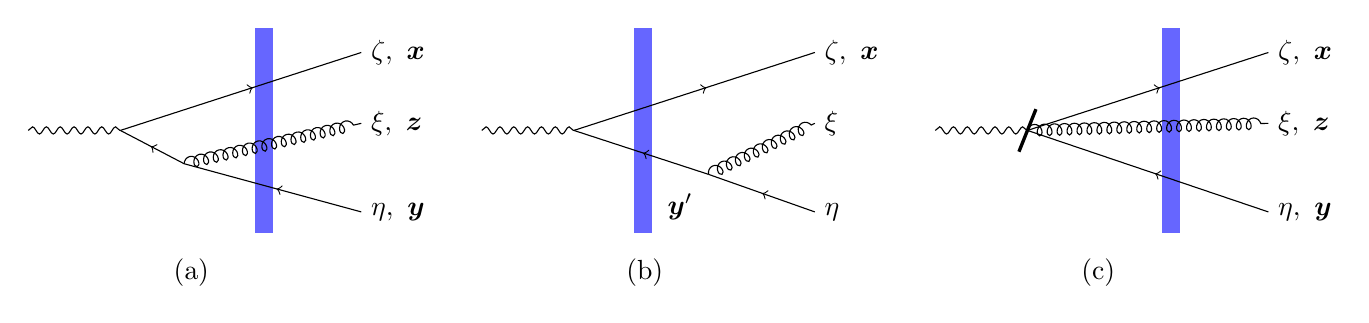
\begin{tikzpicture}[scale=0.9,
  photon/.style={decorate, decoration={snake, amplitude=1.3pt, segment length=5pt}},
  gluon/.style={decorate, decoration={coil, aspect=0.8, amplitude=2.1pt, segment length=3.6pt}},
  fermion/.style={postaction={decorate,decoration={markings,mark=at position 0.55 with {\arrow{>}}}}},
  afermion/.style={postaction={decorate,decoration={markings,mark=at position 0.55 with {\arrow{<}}}}}]
% ---- panel (a): emission before the shockwave ----
\begin{scope}[xshift=0cm]
  \fill[blue!60] (1.9,-1.45) rectangle (2.15,1.45);
  \draw[photon] (-1.3,0) -- (0,0);
  \draw[fermion] (0,0) -- (3.4,1.1) node[right] {$\zeta,\ \vx$};
  \draw[afermion] (0,0) -- (0.9,-0.47);
  \draw[afermion] (0.9,-0.47) -- (3.4,-1.15) node[right] {$\eta,\ \vy$};
  \draw[gluon] (0.9,-0.47) -- (3.4,0.1);
  \node[right] at (3.4,0.1) {$\xi,\ \vz$};
  \node at (1.0,-2.0) {(a)};
\end{scope}
% ---- panel (b): emission after the shockwave ----
\begin{scope}[xshift=6.4cm]
  \fill[blue!60] (0.85,-1.45) rectangle (1.1,1.45);
  \draw[photon] (-1.3,0) -- (0,0);
  \draw[fermion] (0,0) -- (3.4,1.1) node[right] {$\zeta,\ \vx$};
  \draw[afermion] (0,0) -- (1.9,-0.62);
  \draw[afermion] (1.9,-0.62) -- (3.4,-1.15) node[right] {$\eta$};
  \draw[gluon] (1.9,-0.62) -- (3.4,0.1);
  \node[right] at (3.4,0.1) {$\xi$};
  \node at (1.0,-2.0) {(b)};
  \node[below] at (1.5,-0.75) {$\bm{y}'$};
\end{scope}
% ---- panel (c): instantaneous ----
\begin{scope}[xshift=12.8cm]
  \fill[blue!60] (1.9,-1.45) rectangle (2.15,1.45);
  \draw[photon] (-1.3,0) -- (0,0);
  \draw[fermion] (0,0) -- (3.4,1.1) node[right] {$\zeta,\ \vx$};
  \draw[afermion] (0,0) -- (3.4,-1.15) node[right] {$\eta,\ \vy$};
  \draw[gluon] (0,0) -- (3.4,0.1);
  \node[right] at (3.4,0.1) {$\xi,\ \vz$};
  \draw[very thick] (-0.12,-0.3) -- (0.12,0.3);
  \node at (1.0,-2.0) {(c)};
\end{scope}
\end{tikzpicture}
\caption{\small The three topologies contributing to the $q\bar qg$ component of the outgoing
state for gluon emission by the antiquark: (a) regular emission prior to the shockwave (the
blue band), (b) regular emission after the shockwave, (c) the instantaneous vertex, denoted by
the short bar. The quark-emission topologies are obtained by exchanging the roles of the quark
and the antiquark.}
\label{fig:topologies}
\end{figure}

\subsection{Gluon emission by the antiquark prior to the shockwave}
\label{sec:beforeSW}

The contribution of fig.~\ref{fig:topologies}.a to the outgoing state is given by
second-order LCPT as
\begin{align}
\label{eq:pert1}
\ket{\gamma}^{(1)}_{q\bar{q}g} = \ket{q_{2}\bar{q}_{2}g_{2}}
\bra{q_{2}\bar{q}_{2}g_{2}}\hat S\ket{q_{1}\bar{q}_{1}g_{1}}\,
\frac{\bra{q_{1}\bar{q}_{1}g_{1}}H_{\bar{q}g}\ket{q\bar{q}}}
{E_{\bar{q}_{1}}+E_{q_{1}}+E_{g_{1}}-E_{\gamma}}\,
\frac{\bra{q\bar{q}}H_{\gamma\rightarrow q\bar{q}}\ket{\gamma}}{E_{q}+E_{\bar{q}}-E_{\gamma}}\,,
\end{align}
where sums/integrals over the intermediate states are implicit and $\hat S$ is the eikonal
$S$-matrix of the shockwave. We first evaluate eq.~\eqref{eq:pert1} in the absence of
scattering ($\hat S=1$). Using the vertices and energy denominators of
section~\ref{sec:setup}, one finds in transverse momentum space
\begin{align}
\label{eq:wf1mom}
\ket{\gamma_{i}(Q,q^{+},\vq)}^{(1a)}_{q\bar{q}g} & = -\frac{1}{(2\pi)^{6}}
\int d^{2}\kt\, d^{2}\pt \int_{0}^{1} d\zeta \int_{0}^{1-\zeta} d\xi\,
\ket{q^{\alpha}_{\lambda_{1}}(\zeta q^{+},\vk)\,\bar{q}^{\beta}_{\lambda_{2}}(\eta q^{+},\vq-\vk-\vp)\,
g^{a}_{m}(\xi q^{+},\vp)} \notag\\
&\quad\times\frac{e\,e_{f}\,g\,q^{+}\,\zeta(1-\zeta)}{2\sqrt{\xi}\,\big(\kt^{2}+\eps^{2}_{f}\big)}\,
\frac{\Big[\varphi^{ij}_{\lambda_{1}\lambda}(\zeta)\,\kt^{j}
+m_{f}\,\mu^{i}_{\lambda_{1}\lambda}\Big]
\Big[\tau^{mn}_{\lambda\lambda_{2}}(\xi,\eta)\,\pt^{n}
+\xi\,\omega_{f}\,\mu^{m}_{\lambda\lambda_{2}}\Big]\,t^{a}_{\alpha\beta}}
{\zeta(1-\zeta)^{2}\big(\pt^{2}+\omega^{2}_{f}\big)+\xi\eta\big(\kt^{2}+\eps_{f}^{2}\big)}\,,
\end{align}
with the helicity $\lambda$ of the intermediate antiquark implicitly summed over. The
numerator exhibits the four spin structures announced in the Introduction: non-flip/non-flip
($\varphi\tau$), non-flip/flip ($\varphi\mu$), flip/non-flip ($\mu\tau$) and flip/flip
($\mu\mu$).

Wilson lines are diagonal in the transverse coordinate representation, so we Fourier transform
eq.~\eqref{eq:wf1mom},
\begin{align}
\ket{q^{\alpha}_{\lambda_{1}}(\vk)\,\bar q^{\beta}_{\lambda_{2}}(\vq-\vk-\vp)\,g^{a}_{m}(\vp)}
= \int_{\vx,\vy,\vz}\, e^{i\vk\cdot \vx}\, e^{i\vp\cdot \vz}\,
e^{i(\vq-\vk-\vp)\cdot \vy}\,\ket{q^{\alpha}_{\lambda_{1}}(\vx)\,\bar q^{\beta}_{\lambda_{2}}(\vy)\,
g^{a}_{m}(\vz)}\,,
\end{align}
and rewrite the phases in terms of $\kt$ and $\pt$:
\begin{align}
\label{eq:phases}
e^{i[\zeta\vx +\eta \vy + \xi\vz]\cdot \vq}\,e^{-i(\vy-\vz)\cdot \pt}\,
e^{i\left(\vx-\frac{\eta\vy + \xi\vz}{1-\zeta}\right)\cdot \kt}
= e^{i\,\vw\cdot \vq}\, e^{-i\,\vY\cdot \pt}\, e^{i\,\vR\cdot \kt}\,.
\end{align}
The transverse coordinates of the photon ($\vw$) and of the intermediate antiquark ($\vy'$,
prior to the gluon emission) are fixed by the conservation of the centre of energy at the two
vertices,
\begin{align}
\label{eq:wyprime}
\vw = \zeta\vx +(1-\zeta)\,\vy' = \zeta\vx + \eta\vy + \xi\vz\,,\qquad
\vy' = \frac{\eta\,\vy + \xi\,\vz}{1-\zeta}\,,
\end{align}
and the relevant separations are those between the daughter partons at each vertex,
\begin{align}
\label{eq:RY}
\vR \equiv \vx - \vy'\,,\qquad \vY \equiv \vy-\vz\,,\qquad
(1-\zeta)\,\vx - \eta\,\vy -\xi\,\vz = (1-\zeta)\,\vR\,.
\end{align}

In the massless case, the Fourier transform of eq.~\eqref{eq:wf1mom} is a single Bessel
function \cite{Iancu:2022gpw}. With masses, the two denominators in eq.~\eqref{eq:wf1mom}
contain two different scales, $\eps_f$ and $\omega_f$, and there are four numerator structures
to transform, one for each helicity path. We therefore define
\begin{align}
\label{eq:FTdef}
(1-\zeta) \int \frac{d^{2}\kt}{2\pi}\, \frac{d^{2}\pt}{2\pi}\,&
\frac{e^{i\kt\cdot \vR}\, e^{-i\pt\cdot \vY}\;
\big\{\kt^{j}\pt^{n},\ \kt^{j},\ \pt^{n},\ 1\big\}}
{\big(\kt^{2}+\eps^{2}_{f}\big) \big[\zeta(1-\zeta)^{2} \big(\pt^{2}+\omega_{f}^{2}\big)
+ \xi\eta\big(\kt^{2} + \eps^{2}_{f}\big)\big]} \notag\\
&= \Big\{R^{j}Y^{n}\calG^{(11)},\ iR^{j}\calG^{(10)},\ -iY^{n}\calG^{(01)},\ \calG^{(00)}\Big\},
\end{align}
where the functions $\calG^{(\alpha\beta)}=\calG^{(\alpha\beta)}(R,Y)$ depend only upon the
moduli $R=|\vR|$, $Y=|\vY|$ (and on $\zeta,\xi,Q^2,m_f^2$). Combining a Schwinger
parametrisation of the two denominators with the Gaussian transverse integrations (the details
are given in appendix~\ref{app:fourier}), one obtains the four functions as one-dimensional
integrals over a Feynman parameter $u$:
\begin{align}
\label{eq:Gab}
\boxed{\ \ \calG^{(\alpha\beta)}(R,Y) = \frac{a^{\beta}}{2\,\zeta(1-\zeta)}
\int_{0}^{1} \frac{du}{u^{1+\beta}}
\left(\frac{A_{u}}{\Delta_{u}}\right)^{\!\frac{\alpha + \beta}{2}}
K_{\alpha + \beta}\big(\sqrt{A_{u}\Delta_{u}}\big)\,,\qquad \alpha,\beta\in\{0,1\}\,,\ \ }
\end{align}
with $K_\nu$ the modified Bessel function of the second kind, $a$ as in eq.~\eqref{eq:adef},
and
\begin{align}
\label{eq:ADelta}
A_{u} = \eps^{2}_{f} + \frac{u\,\omega^{2}_{f}}{a} =
\zeta(1-\zeta)\,Q^{2} +m^{2}_{f}\left(1+\frac{u\,\zeta\,\xi}{\eta}\right),
\qquad
\Delta_{u} = R^{2} + \frac{a\,Y^{2}}{u}\,.
\end{align}
Explicitly,
\begin{align}
\label{eq:Gexplicit}
\calG^{(11)} &= \frac{a}{2\zeta(1-\zeta)} \int_{0}^{1} \frac{du}{u^{2}}\,
\frac{A_{u}}{\Delta_{u}}\,K_{2}\big(\sqrt{A_{u}\Delta_{u}}\big)\,, &
\calG^{(10)} &= \frac{1}{2\zeta(1-\zeta)} \int_{0}^{1} \frac{du}{u}
\sqrt{\frac{A_{u}}{\Delta_{u}}}\, K_{1}\big(\sqrt{A_{u}\Delta_{u}}\big)\,, \notag\\
\calG^{(01)} &= \frac{a}{2\zeta(1-\zeta)} \int_{0}^{1} \frac{du}{u^{2}}
\sqrt{\frac{A_{u}}{\Delta_{u}}}\, K_{1}\big(\sqrt{A_{u}\Delta_{u}}\big)\,, &
\calG^{(00)} &= \frac{1}{2\zeta(1-\zeta)} \int_{0}^{1} \frac{du}{u}\,
K_{0}\big(\sqrt{A_{u}\Delta_{u}}\big)\,.
\end{align}
The Feynman parameter $u$ interpolates between the two intrinsic scales of the problem: the
endpoint $u\to 1$ is controlled by the overall three-parton virtuality, while the endpoint
$u\to 0$ probes the gluon-emission scale $\omega_f$ at large $aY^2/u$. In the massless limit
$\calG^{(11)}$ collapses to the single Bessel function of \cite{Iancu:2022gpw} while
$\calG^{(10)},\calG^{(01)},\calG^{(00)}$ decouple (their coefficients vanish with $m_f$); see
section~\ref{sec:limits} and appendix~\ref{app:fourier}.

Performing the transform in eq.~\eqref{eq:wf1mom} and attaching the Wilson lines appropriate to
this topology (all three partons cross the shockwave), and subtracting the no-scattering limit,
we arrive at
\begin{align}
\label{eq:wf1}
\ket{\gamma_{i}(Q,q^{+},\vq)}^{(1a)}_{q\bar{q}g} &= -\frac{e\,e_{f}\,g\,q^{+}}{2(2\pi)^{4}}
\int_{\vx,\vy,\vz} \int_{0}^{1} d\zeta \int_{0}^{1-\zeta} d\xi\,
\ket{q^{\alpha}_{\lambda_{1}}(\zeta q^{+},\vx)\,\bar{q}^{\beta}_{\lambda_{2}}(\eta q^{+},\vy)\,
g^{a}_{m}(\xi q^{+},\vz)}\, \frac{\zeta}{\sqrt{\xi}}\, \delta^{(2)}(\vw-\vc) \notag\\
&\quad\times \Psi^{im}_{\lambda_{1}\lambda_{2}}[\calG](\vR,\vY)\;
\Big[U^{ab}(\vz)\,V(\vx)\,t^{b}\,V^{\dagger}(\vy)-t^{a}\Big]_{\alpha\beta}\,,
\end{align}
where $\vc = \zeta\vx +\eta\vy + \xi\vz$ is the centre of energy of the trijet system and the
``effective vertex'' collects the four helicity paths:
\begin{align}
\label{eq:Psidef}
\Psi^{im}_{\lambda_{1}\lambda_{2}}[F] \equiv \sum_{\lambda}
\Big[&\varphi^{ij}_{\lambda_{1}\lambda}(\zeta)\,\tau^{mn}_{\lambda\lambda_{2}}(\xi,\eta)\,
R^{j}Y^{n}\,F^{(11)}
+i\,\xi\,\omega_{f}\,\varphi^{ij}_{\lambda_{1}\lambda}(\zeta)\,\mu^{m}_{\lambda\lambda_{2}}\,
R^{j}\,F^{(10)} \notag\\
&-i\,m_{f}\,\mu^{i}_{\lambda_{1}\lambda}\,\tau^{mn}_{\lambda\lambda_{2}}(\xi,\eta)\,
Y^{n}\,F^{(01)} + m_{f}\,\xi\,\omega_{f}\,
\mu^{i}_{\lambda_{1}\lambda}\,\mu^{m}_{\lambda\lambda_{2}}\,F^{(00)}\Big]\,,
\end{align}
for any quadruplet of radial functions $F^{(\alpha\beta)}$.

\subsection{Gluon emission after the shockwave}
\label{sec:afterSW}

For the topology of fig.~\ref{fig:topologies}.b the only differences with respect to the
previous subsection are the second energy denominator and the Wilson-line structure. The
energy denominator is now the energy difference between the intermediate $q\bar q$ pair and the
final three-parton state, eq.~\eqref{eq:EDemission}, so that
\begin{align}
\frac{1}{\zeta(1-\zeta)^{2}\big(\pt^{2}+\omega^{2}_{f}\big)+\xi\eta\big(\kt^{2}+\eps_{f}^{2}\big)}
\ \longrightarrow\
-\frac{1}{\zeta(1-\zeta)^{2}\big(\pt^{2}+\omega^{2}_{f}\big)}\,,
\end{align}
and the two transverse integrations factorise into standard single-scale transforms,
\begin{align}
\int \frac{d^{2}\kt}{2\pi}\, e^{i\kt\cdot \vR}\,
\frac{\{\kt^{j},1\}}{\kt^{2}+\eps^{2}_{f}}
&= \Big\{\frac{i R^{j}}{R}\,\eps_{f}\,K_{1}(\eps_{f}R),\ K_{0}(\eps_{f} R)\Big\},\notag\\
\int \frac{d^{2}\pt}{2\pi}\, e^{-i\pt\cdot \vY}\,
\frac{\{\pt^{n},1\}}{\pt^{2}+\omega^{2}_{f}}
&= \Big\{-\frac{i Y^{n}}{Y}\,\omega_{f}\,K_{1}(\omega_{f}Y),\ K_{0}(\omega_{f} Y)\Big\}.
\end{align}
With the same normalisation as in eq.~\eqref{eq:FTdef}, the radial functions for this topology
are therefore products of Bessel functions,
\begin{align}
\label{eq:Aab}
\calA^{(11)} = \frac{\eps_{f}K_{1}(\eps_{f} R)}{\zeta(1-\zeta)R}\,
\frac{\omega_{f}K_{1}(\omega_{f}Y)}{Y}\,,\qquad
\calA^{(10)} = \frac{\eps_{f}K_{1}(\eps_{f}R)}{\zeta(1-\zeta)R}\, K_{0}(\omega_{f}Y)\,,\notag\\
\calA^{(01)} = \frac{K_{0}(\eps_{f}R)}{\zeta(1-\zeta)}\,
\frac{\omega_{f}K_{1}(\omega_{f}Y)}{Y}\,,\qquad
\calA^{(00)} = \frac{K_{0}(\eps_{f}R)}{\zeta(1-\zeta)}\,K_{0}(\omega_{f}Y)\,.
\end{align}
Since the gluon is emitted only after the collision, the Wilson lines describe the scattering
of the intermediate $q\bar q$ pair, with transverse coordinates $\vx$ and $\vy'$:
\begin{align}
\label{eq:wf2}
\ket{\gamma_i(\vw)}^{(2)}_{q\bar{q}g} &= +\frac{e\,e_{f}\,g\,q^{+}}{2(2\pi)^{4}}
\int_{\vx,\vy,\vz} \int_{0}^{1} d\zeta \int_{0}^{1-\zeta} d\xi\,
\ket{q^{\alpha}_{\lambda_{1}}(\zeta q^{+},\vx)\,\bar{q}^{\beta}_{\lambda_{2}}(\eta q^{+},\vy)\,
g^{a}_{m}(\xi q^{+},\vz)}\, \frac{\zeta}{\sqrt{\xi}}\, \delta^{(2)}(\vw-\vc) \notag\\
&\quad\times \Psi^{im}_{\lambda_{1}\lambda_{2}}[\calA](\vR,\vY)\;
\Big[V(\vx)\,V^{\dagger}(\vy')\,t^{a}-t^{a}\Big]_{\alpha\beta}\,.
\end{align}
Note that the quark mass makes this contribution more singular at large distances than its
massless counterpart only in appearance: for $\omega_f Y\ll 1$ one has $\omega_f
K_1(\omega_fY)/Y\to 1/Y^2$, recovering the massless behaviour, whereas for $Y\gtrsim
1/\omega_f$ the emission is exponentially cut off --- the scale $\omega_f$ acts as the ``dead
cone'' of the massive emitter in transverse coordinate space.

\subsection{Instantaneous contribution}
\label{sec:inst}

For the instantaneous topology of fig.~\ref{fig:topologies}.c, the single energy denominator
is eq.~\eqref{eq:EDqqbarg} and, by virtue of the identity \eqref{eq:Efidentity}, the Fourier
transform is again elementary:
\begin{align}
\label{eq:GE}
(1-\zeta) \int \frac{d^{2}\kt}{2\pi}\, \frac{d^{2}\pt}{2\pi}\,
\frac{e^{i\kt\cdot \vR}\, e^{-i\pt\cdot \vY}}
{\zeta(1-\zeta)^{2}\big(\pt^{2}+\omega^{2}_{f}\big) + \xi\eta\big(\kt^{2}+\eps^{2}_{f}\big)}
= \frac{E_{f}\,K_{1}(E_{f}\,\calD)}{\calD} \equiv \calG_{E}\,,
\end{align}
where $\calD$ is the same effective transverse size of the three-parton fluctuation as in the
massless case,
\begin{align}
\label{eq:Ddef}
\calD^{2}(\vx,\vy,\vz,\zeta,\xi) = \zeta(1-\zeta)\,\vR^{2} + \frac{\xi\eta\,\vY^{2}}{1-\zeta}
= \zeta\eta\,(\vx-\vy)^{2} + \zeta\xi\,(\vx-\vz)^{2} + \eta\xi\,(\vy-\vz)^{2}\,,
\end{align}
but the virtuality which limits this size is now the mass-shifted scale $E_f$ of
eq.~\eqref{eq:scales}: $E_f\,\calD\lesssim 1$. The corresponding contribution to the outgoing
state reads
\begin{align}
\label{eq:wfinst}
\ket{\gamma_i(\vw)}^{(1\,\text{inst})}_{q\bar{q}g} &= +\frac{e\,e_{f}\,g\,q^{+}}{2(2\pi)^{4}}
\int_{\vx,\vy,\vz} \int_{0}^{1} d\zeta \int_{0}^{1-\zeta} d\xi\,
\ket{q^{\alpha}_{\lambda_{1}}(\zeta q^{+},\vx)\,\bar{q}^{\beta}_{\lambda_{2}}(\eta q^{+},\vy)\,
g^{a}_{m}(\xi q^{+},\vz)}\,\frac{\zeta\,\eta\,\sqrt{\xi}}{1-\zeta}\,\delta^{(2)}(\vw-\vc) \notag\\
&\quad\times \big(\delta^{im}+2i\,\epsilon^{im}\lambda_{1}\big)\,\delta_{\lambda_{1}\lambda_{2}}\,
\calG_E\;\Big[U^{ab}(\vz)\,V(\vx)\,t^{b}\,V^{\dagger}(\vy)-t^{a}\Big]_{\alpha\beta}\,,
\end{align}
with the same Wilson-line structure as in eq.~\eqref{eq:wf1}, as it should (the three partons
exist already at the time of the scattering).

\subsection{Effective vertices and the combined antiquark-emission wave function}
\label{sec:effective}

The three contributions above can be packaged into two effective vertices, one for each
Wilson-line structure,
\begin{align}
\label{eq:M12}
\calM^{im}_{1\,\lambda_{1}\lambda_{2}}(\vx,\vy,\vz,\zeta,\xi) &=
\Psi^{im}_{\lambda_{1}\lambda_{2}}[\calG](\vR,\vY)
- \delta_{\lambda_{1}\lambda_{2}}\,\frac{\xi\eta}{1-\zeta}\,
\big(\delta^{im}+2i\epsilon^{im}\lambda_{1}\big)\,\calG_{E}\,,\notag\\
\calM^{im}_{2\,\lambda_{1}\lambda_{2}}(\vx,\vy,\vz,\zeta,\xi) &=
\Psi^{im}_{\lambda_{1}\lambda_{2}}[\calA](\vR,\vY)\,,
\end{align}
in terms of which all antiquark-emission topologies combine into the single expression
\begin{align}
\label{eq:wfqbar}
\ket{\gamma^{i}(\vw)}_{q\bm{\bar q}g} = -\frac{e\,e_{f}\,g\,q^{+}}{2(2\pi)^{4}}
\int_{\vx,\vy,\vz} \int_{0}^{1} d\zeta \int_{0}^{1-\zeta} d\xi\,&
\ket{q^{\alpha}_{\lambda_{1}}(\zeta q^{+},\vx)\,\bar{q}^{\beta}_{\lambda_{2}}(\eta q^{+},\vy)\,
g^{a}_{m}(\xi q^{+},\vz)}\,\frac{\zeta}{\sqrt{\xi}}\,\delta^{(2)}(\vw-\vc) \notag\\
\times\bigg[\calM^{im}_{1\,\lambda_{1}\lambda_{2}}\,
\Big[U^{ab}(\vz)V(\vx)t^{b}V^{\dagger}(\vy)-t^{a}\Big]_{\alpha\beta}
&- \calM^{im}_{2\,\lambda_{1}\lambda_{2}}\,
\Big[V(\vx)\,V^{\dagger}(\vy')\,t^{a}-t^{a}\Big]_{\alpha\beta}\bigg]\,,
\end{align}
where the boldface label $\bm{\bar q}$ recalls that the antiquark is the emitter. There is no
instantaneous counterpart for the second Wilson structure: the formal substitution
$\vy,\vz\to\vy'$ which generates the after-shockwave colour structure sends $\vY\to 0$, and the
instantaneous term vanishes in this limit.

\subsection{Gluon emission by the quark}
\label{sec:quarkemission}

The contribution where the gluon is emitted by the quark need not be computed anew: it follows
from eq.~\eqref{eq:wfqbar} via symmetry operations which exchange the quark and the antiquark
while keeping the final state fixed \cite{Iancu:2022gpw}: (i) exchange
$\zeta\leftrightarrow\eta$, $\vx\leftrightarrow\vy$, $\alpha\leftrightarrow\beta$,
$\lambda_1\leftrightarrow\lambda_2$; (ii) take the complex conjugate of the vertex structures;
(iii) flip the overall sign (the colour charge of the quark is minus that of the antiquark).
These operations have the following consequences:
\begin{itemize}
\item the intermediate coordinate and separations become
\begin{equation}
\label{eq:quarkcoords}
\vy'\ \to\ \vx' = \frac{\zeta\vx + \xi\vz}{\zeta + \xi}\,,\qquad
\vR\ \to\ \vy-\vx' \equiv -\vRt\,,\qquad
\vY\ \to\ \vx-\vz \equiv \vX\,;
\end{equation}
\item the spinorial structures transform as
\begin{equation}
\varphi^{ij}_{\lambda_{1}\lambda}(\zeta) \to \varphi^{ij\,*}_{\lambda_{2}\lambda}(\eta)
= -\varphi^{ij}_{\lambda\lambda_{2}}(\zeta+\xi)\,,\qquad
\tau^{mn}_{\lambda\lambda_{2}}(\xi,\eta) \to \tau^{mn\,*}_{\lambda\lambda_{1}}(\xi,\zeta)
= \tau^{nm}_{\lambda_{1}\lambda}(\xi,\zeta)\,,
\end{equation}
with $\tau^{mn}_{\lambda\lambda'}(\xi,\zeta)=\delta_{\lambda\lambda'}[(2(1-\eta)-\xi)\delta^{mn}
+2i\xi\epsilon^{mn}\lambda]$, while the helicity-flip pieces map onto
$m_{f}\,\mu^{i}_{\lambda\lambda_{2}}$ and $\xi\,\widetilde\omega_{f}\,\mu^{m}_{\lambda_{1}\lambda}$
with
\begin{equation}
\widetilde\omega_{f} = \frac{\xi\,m_{f}}{1-\eta}\,;
\end{equation}
\item the scales and radial functions are obtained by $\zeta\to\eta$ in the explicit factors:
\begin{align}
\label{eq:quarkscales}
\widetilde\eps^{\,2}_{f} = \eta(1-\eta)Q^{2} + m^{2}_{f}\,,&\qquad
\widetilde a = \frac{\xi\zeta}{\eta(1-\eta)^{2}}\,,\notag\\
\widetilde A_{u} = \eta(1-\eta)Q^{2} + m^{2}_{f}\Big(1+\frac{u\,\eta\,\xi}{\zeta}\Big)\,,&\qquad
\widetilde\Delta_{u} = \vRt^{2} + \frac{\widetilde a\,\vX^{2}}{u}\,,
\end{align}
and $\widetilde\calG^{(\alpha\beta)}(\widetilde R,X)$, $\widetilde\calA^{(\alpha\beta)}
(\widetilde R,X)$ are given by eqs.~\eqref{eq:Gab} and \eqref{eq:Aab} with
$(\zeta,a,A_u,\Delta_u,\eps_f,\omega_f;R,Y)\to(\eta,\widetilde a,\widetilde A_u,
\widetilde\Delta_u,\widetilde\eps_f,\widetilde\omega_f;\widetilde R,X)$. The effective size
$\calD$ of eq.~\eqref{eq:Ddef} is invariant under these operations:
$\calD^2=\eta(1-\eta)\vRt^{2}+\xi\zeta\vX^{2}/(1-\eta)$.
\end{itemize}
The quark-emission effective vertices read
\begin{align}
\label{eq:Psitilde}
\widetilde\Psi^{im}_{\lambda_{1}\lambda_{2}}[F] = \sum_{\lambda}
\Big[&\tau^{nm}_{\lambda_{1}\lambda}(\xi,\zeta)\,\varphi^{ij}_{\lambda\lambda_{2}}(\zeta+\xi)\,
\widetilde R^{j}X^{n}\,F^{(11)}
+i\,\xi\,\widetilde\omega_{f}\,\mu^{m}_{\lambda_{1}\lambda}\,
\varphi^{ij}_{\lambda\lambda_{2}}(\zeta+\xi)\,\widetilde R^{j}\,F^{(10)} \notag\\
&-i\,m_{f}\,\tau^{nm}_{\lambda_{1}\lambda}(\xi,\zeta)\,\mu^{i}_{\lambda\lambda_{2}}\,
X^{n}\,F^{(01)} + m_{f}\,\xi\,\widetilde\omega_{f}\,
\mu^{m}_{\lambda_{1}\lambda}\,\mu^{i}_{\lambda\lambda_{2}}\,F^{(00)}\Big]\,,
\end{align}
together with
\begin{align}
\label{eq:Mtilde12}
\widetilde\calM^{im}_{1\,\lambda_{1}\lambda_{2}} &=
\widetilde\Psi^{im}_{\lambda_{1}\lambda_{2}}[\widetilde\calG](\vRt,\vX)
- \delta_{\lambda_{1}\lambda_{2}}\,\frac{\zeta\xi}{\zeta+\xi}\,
\big(\delta^{im}-2i\epsilon^{im}\lambda_{1}\big)\,\calG_{E}\,,\qquad
\widetilde\calM^{im}_{2\,\lambda_{1}\lambda_{2}} =
\widetilde\Psi^{im}_{\lambda_{1}\lambda_{2}}[\widetilde\calA](\vRt,\vX)\,,
\end{align}
and the full quark-emission wave function is
\begin{align}
\label{eq:wfq}
\ket{\gamma^{i}(\vw)}_{\bm{q}\bar qg} = +\frac{e\,e_{f}\,g\,q^{+}}{2(2\pi)^{4}}
\int_{\vx,\vy,\vz} \int_{0}^{1} d\zeta \int_{0}^{1-\zeta} d\xi\,&
\ket{q^{\alpha}_{\lambda_{1}}(\zeta q^{+},\vx)\,\bar{q}^{\beta}_{\lambda_{2}}(\eta q^{+},\vy)\,
g^{a}_{m}(\xi q^{+},\vz)}\,\frac{\eta}{\sqrt{\xi}}\,\delta^{(2)}(\vw-\vc) \notag\\
\times\bigg[\widetilde\calM^{im}_{1\,\lambda_{1}\lambda_{2}}\,
\Big[U^{ab}(\vz)V(\vx)t^{b}V^{\dagger}(\vy)-t^{a}\Big]_{\alpha\beta}
&- \widetilde\calM^{im}_{2\,\lambda_{1}\lambda_{2}}\,
\Big[t^{a}\,V(\vx')\,V^{\dagger}(\vy)-t^{a}\Big]_{\alpha\beta}\bigg]\,.
\end{align}
Note the position of the colour matrix $t^a$ in the after-shockwave structure: it sits to the
left of the Wilson lines when the emitter is the quark, and to the right when it is the
antiquark, cf.\ eq.~\eqref{eq:wfqbar}. The complete $q\bar qg$ component of the outgoing state
is the sum of eqs.~\eqref{eq:wfqbar} and \eqref{eq:wfq}.

%=====================================================================
\section{The trijet cross-section at leading order}
\label{sec:xsec}

The leading-order cross-section for $q\bar qg$ production is the expectation value of the
product of three number-density operators on the outgoing state constructed in the previous
section:
\begin{align}
\label{eq:xsecdef}
\frac{d\sigma^{\gamma^*_TA\rightarrow q\bar qg}}{dk^+_1 d^{2}\vk_{1}\,dk^+_2 d^{2}\vk_{2}\,
dk^+_3 d^{2}\vk_{3}}\,& (2\pi)\,\delta\big(q^{+}-k^{+}_{1}-k^{+}_{2}-k^{+}_{3}\big) \notag\\
&= \frac{1}{2}\int_{\vw,\bar{\vw}} e^{-i\vq\cdot (\vw-\bar{\vw})}\;
{}_{q\bar{q}g}\!\bra{\gamma^{i}_{T}(\bar{\vw})}
\mathcal{N}_{q}(k_{1})\,\mathcal{N}_{\bar{q}}(k_{2})\,\mathcal{N}_{g}(k_{3})
\ket{\gamma^{i}_{T}(\vw)}_{q\bar{q}g},
\end{align}
where the factor $1/2$ together with the implicit sum over $i$ averages over the transverse
polarisations of the photon, and the CGC average over the target field configurations is
understood. Below we set $\vq=0$ for simplicity. As in \cite{Iancu:2022gpw}, it is natural to
distinguish \emph{direct} contributions, in which the gluon is emitted and reabsorbed by the
same fermion, and \emph{interference} contributions, in which it is emitted by the quark in
the direct amplitude (DA) and reabsorbed by the antiquark in the complex-conjugate amplitude
(CCA), or vice-versa. Transverse coordinates in the CCA carry a bar.

\subsection{Direct contribution: emission by the antiquark}
\label{sec:directqbar}

A direct calculation using eqs.~\eqref{eq:xsecdef} and \eqref{eq:wfqbar} yields
{\small
\begin{align}
\label{eq:xsecqbar}
\frac{d\sigma^{(\bar q),\rm direct}}{d^{3}k_{1}\,d^{3}k_{2}\,d^{3}k_{3}} &=
\frac{e^{2}\,g^{2}\,\zeta^{2}\,C_{F}\,N_{c}}{8\,(2\pi)^{12}\,\xi\,q^{+2}}\,
\Big(\textstyle\sum_{f} e^{2}_{f}\Big)\,
\delta\big(q^{+}-k^{+}_{1}-k^{+}_{2}-k^{+}_{3}\big)
\int_{\vx,\vy,\vz,\vxb,\vyb,\vzb} e^{-i\vk_{1}\cdot (\vx-\vxb)}\,
e^{-i\vk_{2}\cdot (\vy-\vyb)}\, e^{-i\vk_{3}\cdot (\vz-\vzb)} \notag\\
&\quad\times\Big[\calH[\calG;\bar\calG]\,\calW(\vx,\vy,\vz;\vxb,\vyb,\vzb)
-\calH[\calA;\bar\calG]\,\calW(\vx,\vy',\vy';\vxb,\vyb,\vzb) \notag\\
&\qquad\ \,-\calH[\calG;\bar\calA]\,\calW(\vx,\vy,\vz;\vxb,\vyb',\vyb')
+\calH[\calA;\bar\calA]\,\calW(\vx,\vy',\vy';\vxb,\vyb',\vyb')\Big]\,,
\end{align}}

where $d^3k_i\equiv dk_i^+d^2\vk_i$, the sum runs over the active quark flavours, and the
``hard factors'' are the helicity and polarisation sums of products of effective vertices,
\begin{align}
\label{eq:Hdef}
\calH[F;\bar F] \equiv \sum_{\lambda_{1},\lambda_{2}}\sum_{l,r}\,
\calM^{lr}_{\lambda_{1}\lambda_{2}}[F](\vx,\vy,\vz)\;
\calM^{lr\,*}_{\lambda_{1}\lambda_{2}}[\bar F](\vxb,\vyb,\vzb)\,,
\end{align}
with $\calM[\calG]\equiv\calM_1$ and $\calM[\calA]\equiv\calM_2$,
cf.~eq.~\eqref{eq:M12}. Performing the sums (we use
$\sum_i\mu^i\mu^{i*}=2\delta_{\lambda',-\lambda}$ and the fact that helicity-conserving and
helicity-flip paths do not interfere unless they connect the same pair
$(\lambda_1,\lambda_2)$), one finds three types of terms. The regular$\times$regular piece
reads
\begin{align}
\label{eq:Hregreg}
\calH_{\rm reg\times reg}[F;\bar F] &= R^{i}Y^{m}\bar{R}^{j}\bar{Y}^{n}
\Big\{8\big[\eta^{2}+(1-\zeta)^{2}\big]\big[\zeta^{2} + (1-\zeta)^{2}\big]\,
\delta^{ij}\delta^{mn}\notag\\
&\hspace*{2.6cm}-8\,\xi\,(2\zeta - 1)\big(2(1-\zeta)-\xi\big)\,
\epsilon^{ij}\epsilon^{mn}\Big\}\,F^{(11)}\bar{F}^{(11)} \notag\\
&\quad +8\,m^{2}_{f}\big[\eta^{2} + (1-\zeta)^{2}\big]\,(\vY\cdot \bar{\vY})\,
F^{(01)}\bar{F}^{(01)}
+8\,\xi^{2}\omega^{2}_{f}\big[\zeta^{2}+(1-\zeta)^{2}\big]\,(\vR\cdot \bar{\vR})\,
F^{(10)}\bar{F}^{(10)} \notag\\
&\quad + 8\,m^{2}_{f}\,\xi^{2}\omega^{2}_{f}\,F^{(00)}\bar{F}^{(00)} \notag\\
&\quad -8\,\zeta\eta\, m_{f}\,\xi\,\omega_{f}\,
\Big[(\vR\cdot \vY)\,F^{(11)}\bar{F}^{(00)} + (\bar{\vR}\cdot \bar{\vY})\,F^{(00)}\bar{F}^{(11)}
\notag\\
&\hspace*{3.2cm} + (\vR\cdot \bar{\vY})\,F^{(10)}\bar{F}^{(01)}
+ (\vY\cdot \bar{\vR})\,F^{(01)}\bar{F}^{(10)}\Big]\,,
\end{align}
the regular$\times$instantaneous interference (plus its hermitian conjugate) is
\begin{align}
\label{eq:Hreginst}
\calH_{\rm reg\times inst}[F;\bar F] = -\frac{8\,\zeta\,\xi\,\eta^{2}}{1-\zeta}\,
\Big[(\vR\cdot \vY)\,F^{(11)}\,\bar{\calG}_{E} + (\bar{\vR}\cdot \bar{\vY})\,\calG_{E}\,
\bar{F}^{(11)}\Big]
+\frac{8\,\xi^{2}\,\eta\,m_{f}\,\omega_{f}}{1-\zeta}\,
\Big[F^{(00)}\,\bar{\calG}_{E} + \calG_{E}\,\bar{F}^{(00)}\Big]\,,
\end{align}
and the instantaneous$\times$instantaneous piece is
\begin{align}
\label{eq:Hinstinst}
\calH_{\rm inst\times inst} = 8\left[\frac{\xi\,\eta}{1-\zeta}\right]^{2}
\calG_{E}\,\bar{\calG}_{E}\,.
\end{align}
The first line of eq.~\eqref{eq:Hregreg} is the massless result of \cite{Iancu:2022gpw}
(their eq.~(5.5)); all the other terms are new. Note in particular the last line of
eq.~\eqref{eq:Hregreg}, which describes the interference between the double-flip path
($F^{(00)}$) and the non-flip path ($F^{(11)}$), as well as between the two single-flip paths:
it is linear in $m_f\,\omega_f\propto m_f^2$, as it must, since a single helicity flip cannot
interfere with a non-flip amplitude. Also the second term in eq.~\eqref{eq:Hreginst} is a pure
mass effect: the instantaneous vertex is helicity conserving, so it now interferes with the
double-flip ($F^{(00)}$) path as well.

The effects of the collision are encoded in the function $\calW$, defined as the linear
combination of partonic $S$-matrices
\begin{align}
\label{eq:Wdef}
\calW(\vx,\vy,\vz;\vxb,\vyb,\vzb) \equiv
S_{q\bar{q}g\,q\bar{q}g}(\vx,\vy,\vz;\vxb,\vyb,\vzb)
-S_{q\bar{q}g}(\vx,\vy,\vz) - S^{\dagger}_{q\bar{q}g}(\vxb,\vyb,\vzb) + 1\,,
\end{align}
where $S_{q\bar qg\,q\bar qg}$ describes the scattering of the three-parton system in both the
DA and the CCA, and $S_{q\bar qg}$ ($S^\dagger_{q\bar qg}$) the case where the scattering
occurs in the DA (CCA) only. Using Fierz identities to trade the adjoint Wilson lines for
fundamental ones, and taking the large-$N_c$ limit, these reduce to products of dipoles and
quadrupoles \cite{Iancu:2022gpw},
\begin{equation}
\calS(\vx,\vy)\equiv\frac{1}{N_{c}}\big\langle{\rm tr}\big[V(\vx)V^{\dagger}(\vy)\big]
\big\rangle\,,\qquad
\calQ(\vx_{1},\vx_{2},\vx_{3},\vx_{4})\equiv\frac{1}{N_{c}}\big\langle{\rm tr}
\big[V(\vx_{1})V^{\dagger}(\vx_{2})V(\vx_{3})V^{\dagger}(\vx_{4})\big]\big\rangle\,,
\end{equation}
namely
\begin{align}
\label{eq:W1}
\calW(\vx,\vy,\vz;\vxb,\vyb,\vzb) \simeq \calQ(\vx,\vz,\vzb,\vxb)\, \calQ(\vz,\vy,\vyb,\vzb)
- \calS(\vx,\vz)\,\calS(\vz,\vy) - \calS(\vzb,\vxb)\,\calS(\vyb,\vzb) +1\,.
\end{align}
The ``subtracted'' colour structures, in which the scattering of the three-parton system in
the DA and/or the CCA is replaced by that of the effective $q\bar q$ pair, are obtained from
eq.~\eqref{eq:W1} by the appropriate coincidence limits:
\begin{align}
\label{eq:W234}
\calW(\vx,\vy',\vy';\vxb,\vyb,\vzb) &\simeq \calQ(\vx,\vy',\vzb,\vxb)\,\calS(\vyb,\vzb)
- \calS(\vx,\vy') - \calS(\vzb,\vxb)\,\calS(\vyb,\vzb) +1\,,\notag\\
\calW(\vx,\vy,\vz;\vxb,\vyb',\vyb') &\simeq \calQ(\vx,\vz,\vyb',\vxb)\,\calS(\vz,\vy)
- \calS(\vx,\vz)\,\calS(\vz,\vy) - \calS(\vyb',\vxb) +1\,,\notag\\
\calW(\vx,\vy',\vy';\vxb,\vyb',\vyb') &\simeq \calQ(\vx,\vy',\vyb',\vxb)
-\calS(\vx,\vy') - \calS(\vyb',\vxb) +1\,.
\end{align}
The last structure is the same as for the leading-order $q\bar q$ production, as expected: it
corresponds to graphs where the gluon is emitted and reabsorbed after the collision in both
the DA and the CCA. The quark mass does not modify any of these colour structures --- it only
changes the hard factors which multiply them.

\subsection{Direct contribution: emission by the quark}
\label{sec:directq}

The direct contribution where the gluon is emitted and reabsorbed by the quark follows from
the symmetry operations of section~\ref{sec:quarkemission}:
{\small
\begin{align}
\label{eq:xsecq}
\frac{d\sigma^{(q),\rm direct}}{d^{3}k_{1}\,d^{3}k_{2}\,d^{3}k_{3}} &=
\frac{e^{2}\,g^{2}\,\eta^{2}\,C_{F}\,N_{c}}{8\,(2\pi)^{12}\,\xi\,q^{+2}}\,
\Big(\textstyle\sum_{f} e^{2}_{f}\Big)\,
\delta\big(q^{+}-k^{+}_{1}-k^{+}_{2}-k^{+}_{3}\big)
\int_{\vx,\vy,\vz,\vxb,\vyb,\vzb} e^{-i\vk_{1}\cdot (\vx-\vxb)}\,
e^{-i\vk_{2}\cdot (\vy-\vyb)}\, e^{-i\vk_{3}\cdot (\vz-\vzb)} \notag\\
&\quad\times\Big[\widetilde\calH[\widetilde\calG;\bar{\widetilde\calG}]\,
\calW(\vy,\vx,\vz;\vyb,\vxb,\vzb)
-\widetilde\calH[\widetilde\calA;\bar{\widetilde\calG}]\,\calW(\vy,\vx',\vx';\vyb,\vxb,\vzb) \notag\\
&\qquad\ \ -\widetilde\calH[\widetilde\calG;\bar{\widetilde\calA}]\,\calW(\vy,\vx,\vz;\vyb,\vxb',\vxb')
+\widetilde\calH[\widetilde\calA;\bar{\widetilde\calA}]\,\calW(\vy,\vx',\vx';\vyb,\vxb',\vxb')\Big],
\end{align}}

with $\widetilde\calH$ built from the vertices \eqref{eq:Mtilde12} in full analogy with
eq.~\eqref{eq:Hdef}. The explicit sums read
\begin{align}
\label{eq:Htregreg}
\widetilde\calH_{\rm reg\times reg} &= \widetilde R^{i} X^{m} \bar{\widetilde R}^{j}\bar{X}^{n}
\Big\{8\big[\zeta^{2} + (1-\eta)^{2}\big]\big[\eta^{2} + (1-\eta)^{2}\big]\,
\delta^{ij}\delta^{mn}\notag\\
&\hspace*{2.6cm}- 8\,\xi\, (2\eta -1)\big(2(1-\eta)-\xi\big)\,
\epsilon^{ij}\epsilon^{mn}\Big\}\,F^{(11)}\bar{F}^{(11)} \notag\\
&\quad +8m^{2}_{f}\big[\zeta^{2} + (1-\eta)^{2}\big] (\vX\cdot \bar{\vX})\,F^{(01)}\bar{F}^{(01)}
+ 8\xi^{2}\widetilde\omega^{2}_{f}\big[\eta^{2}+(1-\eta)^{2}\big]
(\vRt\cdot \bar{\vRt})\,F^{(10)}\bar{F}^{(10)} \notag\\
&\quad +8m^{2}_{f}\xi^{2}\widetilde\omega^{2}_{f}\,F^{(00)}\bar{F}^{(00)} \notag\\
&\quad +8\,\zeta\eta\, m_{f}\, \xi\, \widetilde\omega_{f}\,
\Big[(\vRt\cdot \vX)\, F^{(11)}\bar{F}^{(00)} + (\bar{\vRt}\cdot \bar{\vX})\,F^{(00)}\bar{F}^{(11)}
\notag\\
&\hspace*{3.2cm} + (\vRt\cdot \bar{\vX})\,F^{(10)}\bar{F}^{(01)}
+ (\vX\cdot \bar{\vRt})\,F^{(01)}\bar{F}^{(10)}\Big]\,,
\end{align}
\begin{align}
\label{eq:Htreginst}
\widetilde\calH_{\rm reg\times inst} = \frac{8\,\zeta^{2}\,\xi\,\eta}{1-\eta}
\Big[(\vRt\cdot \vX)\,F^{(11)}\,\bar{\calG}_{E} + (\bar{\vRt}\cdot \bar{\vX})\,
\calG_{E}\,\bar{F}^{(11)}\Big]
+ \frac{8\,\xi^{2}\,\zeta\,m_{f}\,\widetilde\omega_{f}}{1-\eta}\,
\Big[F^{(00)}\,\bar{\calG}_{E} + \calG_{E}\,\bar{F}^{(00)}\Big]\,,
\notag\\
\widetilde\calH_{\rm inst\times inst} = 8\left[\frac{\xi\,\zeta}{1-\eta}\right]^{2}
\calG_{E}\,\bar{\calG}_{E}\,,
\end{align}
where it is understood that $F^{(\alpha\beta)}=\widetilde\calG^{(\alpha\beta)}$ or
$\widetilde\calA^{(\alpha\beta)}$ according to the term considered in eq.~\eqref{eq:xsecq}.
Observe the sign flip of the $F^{(11)}\bar F^{(00)}$-type interference terms relative to the
antiquark case, eq.~\eqref{eq:Hregreg}: it originates from the complex conjugation of the
helicity structures under the quark--antiquark exchange. The colour structures are obtained
from eqs.~\eqref{eq:W1}--\eqref{eq:W234} by the relabelling appropriate to a gluon emitted off
the quark line, e.g.
\begin{align}
\calW(\vy,\vx,\vz;\vyb,\vxb,\vzb) \simeq \calQ(\vy,\vz,\vzb,\vyb)\, \calQ(\vz,\vx,\vxb,\vzb)
- \calS(\vy,\vz)\,\calS(\vz,\vx) - \calS(\vzb,\vyb)\,\calS(\vxb,\vzb) +1\,,
\end{align}
and similarly for the subtracted terms, with $\vy',\vyb'$ replaced by $\vx',\vxb'$.

\subsection{Interference contributions}
\label{sec:interference}

Finally, in the interference terms the gluon is emitted by the quark in the DA and reabsorbed
by the antiquark in the CCA (plus the complex-conjugate configuration, accounted for by the
factor $2\,{\mathcal Re}$):
{\small
\begin{align}
\label{eq:xseccross}
\frac{d\sigma^{\rm inter}}{d^{3}k_{1}\,d^{3}k_{2}\,d^{3}k_{3}} &=
-\frac{e^{2}\,g^{2}\,\eta\,\zeta\,C_{F}\,N_{c}}{8\,(2\pi)^{12}\,\xi\,q^{+2}}\,
\Big(\textstyle\sum_{f} e^{2}_{f}\Big)\,
\delta\big(q^{+}-k^{+}_{1}-k^{+}_{2}-k^{+}_{3}\big)\notag\\
&\quad\times 2\,{\mathcal Re}
\int_{\vx,\vy,\vz,\vxb,\vyb,\vzb} e^{-i\vk_{1}\cdot (\vx-\vxb)}\,
e^{-i\vk_{2}\cdot (\vy-\vyb)}\, e^{-i\vk_{3}\cdot (\vz-\vzb)} \notag\\
&\quad\times\Big[\calH^{\times}[\widetilde\calG;\bar{\calG}]\,
\calW(\vx,\vy,\vz;\vxb,\vyb,\vzb) \notag\\
&\qquad\ \,-\calH^{\times}[\widetilde\calA;\bar{\calG}]\,\calW(\vx',\vy,\vx';\vxb,\vyb,\vzb) \notag\\
&\qquad\ \,-\calH^{\times}[\widetilde\calG;\bar{\calA}]\,\calW(\vx,\vy,\vz;\vxb,\vyb',\vyb')
\notag\\
&\qquad\ \,+\calH^{\times}[\widetilde\calA;\bar{\calA}]\,\calW(\vx',\vy,\vx';\vxb,\vyb',\vyb')\Big],
\end{align}}

with the mixed hard factor
\begin{align}
\calH^{\times}[\widetilde F;\bar F] \equiv \sum_{\lambda_{1},\lambda_{2}}\sum_{l,r}
\widetilde{\calM}^{lr}_{\lambda_{1}\lambda_{2}}[\widetilde F](\vx,\vy,\vz)\;
\calM^{lr\,*}_{\lambda_{1}\lambda_{2}}[\bar F](\vxb,\vyb,\vzb)\,.
\end{align}
The helicity sums yield
\begin{align}
\label{eq:Hxregreg}
\calH^{\times}_{\rm reg\times reg} &= \widetilde R^{i}X^{m}\bar{R}^{j}\bar{Y}^{n}
\Big\{8\big[1-\xi-2\zeta\eta\big]\big[\xi(1-\xi) + 2\zeta\eta\big]\,\delta^{ij}\delta^{mn}\notag\\
&\hspace*{2.6cm}-8\,\xi\,\big[1-2\zeta-\xi\big]^{2}\,\epsilon^{ij}\epsilon^{mn}\Big\}\,
\widetilde F^{(11)}\bar{F}^{(11)} \notag\\
&\quad +8\,m^{2}_{f}\,(\xi +2\zeta\eta)\, (\vX\cdot \bar{\vY})\,
\widetilde F^{(01)}\bar{F}^{(01)}
- 8\,(\xi + 2\eta\zeta)\,\xi^{2}\,\widetilde\omega_{f}\,\omega_{f}\,
(\vRt\cdot\bar{\vR})\,\widetilde F^{(10)}\bar{F}^{(10)} \notag\\
&\quad - 8\,(\zeta + \xi)^{2}\,m_{f}\,\xi\,\omega_{f}\,(\vRt\cdot \vX)\,
\widetilde F^{(11)}\bar{F}^{(00)}
+ 8\,(1-\zeta)^{2}\,m_{f}\,\xi\,\widetilde\omega_{f}\,(\bar{\vR}\cdot \bar{\vY})\,
\widetilde F^{(00)}\bar{F}^{(11)} \notag\\
&\quad +8\,\eta^{2}\,m_{f}\,\xi\, \widetilde\omega_{f}\,(\vRt\cdot \bar{\vY})\,
\widetilde F^{(10)}\,\bar{F}^{(01)}
-8\,\zeta^{2}\,m_{f}\,\xi\,\omega_{f}\,(\vX\cdot \bar{\vR})\,
\widetilde F^{(01)}\bar{F}^{(10)}\,,
\end{align}
\begin{align}
\label{eq:Hxreginst}
\calH^{\times}_{\rm reg\times inst} = -\frac{8\,\xi\,\eta\, (\xi +\zeta)^{2}}{1-\zeta}\,
(\vRt\cdot \vX)\,\widetilde F^{(11)}\,\bar{\calG}_{E}
+ \frac{8\,\xi\,\zeta\,(1-\zeta)^{2}}{\xi + \zeta}\,(\bar{\vR}\cdot \bar{\vY})\,
\calG_{E}\,\bar{F}^{(11)}\,,
\qquad
\calH^{\times}_{\rm inst\times inst} = 0\,,
\end{align}
the vanishing of the instantaneous$\times$instantaneous interference being a consequence of
the opposite transverse-spin structures, $\sum_{l,r}(\delta^{lr}-2i\epsilon^{lr}\lambda_{1})
(\delta^{lr}+2i\epsilon^{lr}\lambda_{1})^{*} = 0$ for $\lambda_1=\pm 1/2$. The massless piece
(first line of eq.~\eqref{eq:Hxregreg}) coincides with eq.~(5.17) of \cite{Iancu:2022gpw}.
Note that in the interference the mass terms are no longer organised in pairs: e.g.\ the
$\widetilde F^{(11)}\bar F^{(00)}$ coefficient involves $\omega_f$ (the antiquark-side scale)
while $\widetilde F^{(00)}\bar F^{(11)}$ involves $\widetilde\omega_f$, reflecting the
different emitters in the DA and the CCA.

The colour structures in eq.~\eqref{eq:xseccross} are again products of dipoles and
quadrupoles at large $N_c$:
\begin{align}
\label{eq:Wcross}
\calW(\vx',\vy,\vx';\vxb,\vyb,\vzb) &\simeq \calS(\vzb,\vxb)\,\calQ(\vx',\vy,\vyb,\vzb)
- \calS(\vx',\vy) - \calS(\vzb,\vxb)\,\calS(\vyb,\vzb) + 1\,,\notag\\
\calW(\vx',\vy,\vx';\vxb,\vyb',\vyb') &\simeq \calS(\vyb',\vxb)\, \calS(\vx',\vy)
- \calS(\vx',\vy) - \calS(\vyb',\vxb) +1\,,
\end{align}
together with $\calW(\vx,\vy,\vz;\vxb,\vyb,\vzb)$ and $\calW(\vx,\vy,\vz;\vxb,\vyb',\vyb')$
already shown in eqs.~\eqref{eq:W1}--\eqref{eq:W234}. For the numerical evaluation of all
these colour correlators one may rely on the Gaussian approximation for the CGC averages, in
which each quadrupole is expressed in terms of dipoles only; the complete set of the resulting
expressions is collected in appendix~\ref{app:gaussian}.

%=====================================================================
\section{The cross-section in momentum space: elastic contribution}
\label{sec:momspace}

For many purposes --- in particular for studying azimuthal correlations and the approach to
the back-to-back limit --- it is useful to have the cross-section directly in transverse
momentum space. In this section we perform the Fourier transform explicitly for the
\emph{elastic} part of the colour structure, i.e.\ the piece of eqs.~\eqref{eq:W1},
\eqref{eq:W234} and \eqref{eq:Wcross} in which each quadrupole is replaced by the product of
the dipole built from its DA coordinates and the dipole built from its CCA coordinates,
$\calQ(\vx,\vz,\vzb,\vxb)\to \calS(\vx,\vz)\,\calS(\vzb,\vxb)$, etc. This is the leading term
of the Gaussian decomposition of appendix~\ref{app:gaussian}, for which the DA and the CCA
scatter independently and the six-point colour structure factorises,
\begin{align}
\label{eq:Welastic}
\calW(\vx,\vy,\vz;\vxb,\vyb,\vzb)\Big|_{\rm el} =
\big[\calS(\vx,\vz)\,\calS(\vz,\vy)-1\big]\big[\calS(\vzb,\vxb)\,\calS(\vyb,\vzb)-1\big],
\end{align}
and similarly for the other thirteen colour structures (the subtracted terms factorise
exactly in the same way, with the appropriate coincidence limits). For a homogeneous target
of transverse area $\Spe$, the dipole depends only on the coordinate difference and we define
\begin{align}
\label{eq:Dldef}
\calS(\bm a,\bm b) = \int\frac{d^{2}\vl}{(2\pi)^{2}}\,e^{i\vl\cdot(\bm a-\bm b)}\,
\calD(\vl)\,,\qquad
\calD(\vl) = \int d^{2}\bm r\,e^{-i\vl\cdot \bm r}\,\calS(\bm r)\,,\qquad
\int\frac{d^{2}\vl}{(2\pi)^{2}}\,\calD(\vl)=\calS(0)=1\,.
\end{align}

\subsection{Change of variables and relative momenta}

For the antiquark-emission terms we trade $(\vx,\vy,\vz)$ for $(\vc,\vR,\vY)$ --- the centre
of energy and the two relative separations of eqs.~\eqref{eq:wyprime}--\eqref{eq:RY} --- with
unit Jacobian:
\begin{align}
\vx = \vc+(1-\zeta)\vR,\qquad \vy = \vc-\zeta \vR+\frac{\xi}{1-\zeta}\vY,\qquad
\vz = \vc-\zeta \vR-\frac{\eta}{1-\zeta}\vY,\qquad \vy' = \vc-\zeta \vR\,,
\end{align}
so that the dipole arguments become
\begin{align}
\vx-\vz = \vR+\frac{\eta}{1-\zeta}\,\vY,\qquad \vz-\vy=-\vY,\qquad \vx-\vy' = \vR\,.
\end{align}
For the quark-emission terms we use instead $(\vc,\vRt,\vX)$, cf.~eq.~\eqref{eq:quarkcoords}:
\begin{align}
\vy = \vc-(1-\eta)\vRt,\qquad \vx = \vc+\eta\vRt+\frac{\xi}{1-\eta}\vX,\qquad
\vz = \vc+\eta\vRt-\frac{\zeta}{1-\eta}\vX,\qquad \vx' = \vc+\eta\vRt\,,
\end{align}
with $\vx-\vz = \vX$, $\vz-\vy = \vRt-\frac{\zeta}{1-\eta}\vX$, $\vx'-\vy=\vRt$. The phase of
the cross-section separates accordingly,
\begin{align}
\label{eq:phase}
\vk_{1}\cdot \vx+\vk_{2}\cdot \vy+\vk_{3}\cdot \vz =
(\vk_{1}+\vk_{2}+\vk_{3})\cdot \vc+\kt\cdot \vR-\pt\cdot \vY
= (\vk_{1}+\vk_{2}+\vk_{3})\cdot \vc+\ktq\cdot\vRt-\ptq\cdot \vX\,,
\end{align}
with the relative momenta conjugate to the separations,
\begin{align}
\label{eq:relmom}
\kt = (1-\zeta)\vk_{1}-\zeta(\vk_{2}+\vk_{3})\,,&\qquad
\pt=\frac{\eta\,\vk_{3}-\xi\,\vk_{2}}{1-\zeta}\,,\notag\\
\ktq = \eta(\vk_{1}+\vk_{3})-(1-\eta)\vk_{2}\,,&\qquad
\ptq = \frac{\zeta\,\vk_{3}-\xi\,\vk_{1}}{1-\eta}\,.
\end{align}
The integral over $\vc$ produces the overall transverse momentum conservation (recall that we
set $\vq=0$), while the homogeneity of the target produces the factor $\Spe$.

\subsection{Wave functions in momentum space}

Inverting the Fourier transforms which defined the radial functions in
section~\ref{sec:wf}, the effective vertices can be written as
\begin{align}
\calM^{lr}_{1,2}(\vR,\vY) = \int\frac{d^{2}\kt}{2\pi}\frac{d^{2}\pt}{2\pi}\,
e^{i\kt\cdot \vR-i\pt\cdot \vY}\,\Phi^{lr}_{1,2}(\kt,\pt)\,,
\end{align}
with (helicity labels suppressed)
\begin{align}
\label{eq:Phidef}
\Phi^{lr}_{1}(\vk,\vp) & = N^{lr}(\vk,\vp)\,f_{1}(\vk,\vp)
-\xi\eta\,\big(\delta^{lr}+2i\epsilon^{lr}\lambda_{1}\big)\delta_{\lambda_{1}\lambda_{2}}\,
g(\vk,\vp)\,,\qquad
\Phi^{lr}_{2}(\vk,\vp) = N^{lr}(\vk,\vp)\,f_{2}(\vk,\vp)\,,
\end{align}
where the numerator collects the four spin structures,
\begin{align}
\label{eq:Ndef}
N^{lr}_{\lambda_{1}\lambda_{2}}(\vk,\vp) = \sum_{\lambda}
\Big[\varphi^{lj}_{\lambda_{1}\lambda}(\zeta)\,k^{j}+m_{f}\,\mu^{l}_{\lambda_{1}\lambda}\Big]
\Big[\tau^{rn}_{\lambda\lambda_{2}}(\xi,\eta)\,p^{n}+\xi\,\omega_{f}\,
\mu^{r}_{\lambda\lambda_{2}}\Big]\,,
\end{align}
and the scalar propagator functions are
\begin{align}
\label{eq:fg}
f_{1}(\vk,\vp) & = \frac{1-\zeta}{\big(\vk^{2}+\eps^{2}_{f}\big)
\big[\zeta(1-\zeta)^{2}\big(\vp^{2}+\omega^{2}_{f}\big)
+\xi\eta\big(\vk^{2}+\eps^{2}_{f}\big)\big]}\,,\notag\\
g(\vk,\vp) & = \frac{1}{\zeta(1-\zeta)^{2}\big(\vp^{2}+\omega^{2}_{f}\big)
+\xi\eta\big(\vk^{2}+\eps^{2}_{f}\big)}\,,\qquad
f_{2}(\vk,\vp) = \frac{1}{\zeta(1-\zeta)\big(\vk^{2}+\eps^{2}_{f}\big)
\big(\vp^{2}+\omega^{2}_{f}\big)}\,.
\end{align}
The quark-emission vertices $\widetilde\Phi^{lr}_{1,2}(\ktq,\ptq)$ have the same structure,
with the numerator
$\widetilde N^{lr}_{\lambda_1\lambda_2}=\sum_\lambda[\tau^{nr}_{\lambda_{1}\lambda}(\xi,\zeta)
p^{n}+\xi\widetilde\omega_{f}\mu^{r}_{\lambda_{1}\lambda}]
[\varphi^{lj}_{\lambda\lambda_{2}}(\zeta+\xi)k^{j}+m_{f}\mu^{l}_{\lambda\lambda_{2}}]$, the
instantaneous structure $(\delta^{lr}-2i\epsilon^{lr}\lambda_{1})$ with coefficient
$\xi\zeta\,\widetilde g$, and $\widetilde f_{1},\widetilde f_{2},\widetilde g$ obtained from
eq.~\eqref{eq:fg} by $(1-\zeta)\to(1-\eta)$, $\xi\eta\to\xi\zeta$,
$\zeta(1-\zeta)\to\eta(1-\eta)$, $\eps_f\to\widetilde\eps_f$, $\omega_f\to\widetilde\omega_f$.

\subsection{Scattering as convolutions and the reduced amplitudes}

In the elastic approximation each dipole factor $\calS$ translates, via
eq.~\eqref{eq:Dldef}, into a convolution of the momentum-space vertex with the distribution
$\calD(\vl)$. Explicitly,
\begin{align}
\label{eq:convolutions}
\int d^{2}\vR\,d^{2}\vY\,e^{-i\kt\cdot \vR+i\pt\cdot \vY}\,\calM_{1}\,
\calS(\vx,\vz)\,\calS(\vz,\vy) & = (2\pi)^{2}\int_{\vl_{1},\vl_{2}}
\calD(\vl_{1})\,\calD(\vl_{2})\;\Phi_{1}\Big(\kt-\vl_{1},\,
\pt+\tfrac{\eta}{1-\zeta}\vl_{1}-\vl_{2}\Big)\,,\notag \\
\int d^{2}\vR\,d^{2}\vY\,e^{-i\kt\cdot \vR+i\pt\cdot \vY}\,\calM_{2}\,
\calS(\vx,\vy') & = (2\pi)^{2}\int_{\vl_{1}}\calD(\vl_{1})\;
\Phi_{2}\big(\kt-\vl_{1},\,\pt\big)\,,\notag \\
\int d^{2}\vRt\,d^{2}\vX\,e^{-i\ktq\cdot\vRt+i\ptq\cdot \vX}\,\widetilde{\calM}_{1}\,
\calS(\vx,\vz)\,\calS(\vz,\vy) & = (2\pi)^{2}\int_{\vl_{1},\vl_{2}}
\calD(\vl_{1})\,\calD(\vl_{2})\;\widetilde{\Phi}_{1}\Big(\ktq-\vl_{2},\,
\ptq+\vl_{1}-\tfrac{\zeta}{1-\eta}\vl_{2}\Big)\,,\notag \\
\int d^{2}\vRt\,d^{2}\vX\,e^{-i\ktq\cdot\vRt+i\ptq\cdot \vX}\,\widetilde{\calM}_{2}\,
\calS(\vx',\vy) & = (2\pi)^{2}\int_{\vl_{2}}\calD(\vl_{2})\;
\widetilde{\Phi}_{2}\big(\ktq-\vl_{2},\,\ptq\big)\,,
\end{align}
with $\int_{\vl}\equiv\int d^2\vl/(2\pi)^2$. The shifted arguments have a transparent
physical interpretation: on the support of $\delta^{(2)}(\vk_1+\vk_2+\vk_3)$ they are simply
the relative momenta constructed from the parton momenta \emph{prior} to the scattering,
$\vk_{1}-\vl_{1}$, $\vk_{2}+\vl_{2}$ and $\vk_{3}+\vl_{1}-\vl_{2}$:
\begin{align}
\label{eq:kapparho}
\bm\kappa \equiv \kt-\vl_{1} = \vk_{1}-\vl_{1}\,, &\qquad
\bm\rho \equiv \pt+\tfrac{\eta}{1-\zeta}\,\vl_{1}-\vl_{2}
= (\vk_{3}+\vl_{1}-\vl_{2})+\tfrac{\xi}{1-\zeta}(\vk_{1}-\vl_{1})\,,\notag \\
\bm\kappa_{q} \equiv \ktq-\vl_{2} = -(\vk_{2}+\vl_{2})\,, &\qquad
\bm\rho_{q} \equiv \ptq+\vl_{1}-\tfrac{\zeta}{1-\eta}\,\vl_{2}
= (\vk_{3}+\vl_{1}-\vl_{2})+\tfrac{\xi}{1-\eta}(\vk_{2}+\vl_{2})\,.
\end{align}
That is, $\vl_1$ and $\vl_2$ are the transverse momenta transferred by the shockwave to the
two effective dipoles.

It is now convenient to introduce reduced amplitudes which combine, for each spin structure,
the two Wilson-line topologies of the DA together with their no-scattering subtractions
(we use $\int_{\vl}\calD(\vl)=1$ to write the single convolutions under the double one):
\begin{align}
\label{eq:Tdef}
T^{jn} & = \int_{\vl_{1},\vl_{2}}\calD(\vl_{1})\calD(\vl_{2})
\Big[\kappa^{j}\rho^{n}\,f_{1}(\bm\kappa,\bm\rho)
-\kappa^{j}\pt^{n}\,f_{2}(\bm\kappa,\pt)\Big]
-\kt^{j}\pt^{n}\Big[f_{1}(\kt,\pt)-f_{2}(\kt,\pt)\Big]\,,\notag \\
T^{j}_{k} & = \int_{\vl_{1},\vl_{2}}\calD(\vl_{1})\calD(\vl_{2})
\Big[\kappa^{j}\,f_{1}(\bm\kappa,\bm\rho)-\kappa^{j}\,f_{2}(\bm\kappa,\pt)\Big]
-\kt^{j}\Big[f_{1}(\kt,\pt)-f_{2}(\kt,\pt)\Big]\,,\notag \\
T^{n}_{p} & = \int_{\vl_{1},\vl_{2}}\calD(\vl_{1})\calD(\vl_{2})
\Big[\rho^{n}\,f_{1}(\bm\kappa,\bm\rho)-\pt^{n}\,f_{2}(\bm\kappa,\pt)\Big]
-\pt^{n}\Big[f_{1}(\kt,\pt)-f_{2}(\kt,\pt)\Big]\,,\notag \\
T_{0} & = \int_{\vl_{1},\vl_{2}}\calD(\vl_{1})\calD(\vl_{2})
\Big[f_{1}(\bm\kappa,\bm\rho)-f_{2}(\bm\kappa,\pt)\Big]
-\Big[f_{1}(\kt,\pt)-f_{2}(\kt,\pt)\Big]\,,\notag\\
T_{I} & = \int_{\vl_{1},\vl_{2}}\calD(\vl_{1})\calD(\vl_{2})\,g(\bm\kappa,\bm\rho)
-g(\kt,\pt)\,,
\end{align}
and similarly $\widetilde T^{jn},\widetilde T^{j}_{k},\widetilde T^{n}_{p},\widetilde T_{0},
\widetilde T_{I}$ for the quark emission, with
$(\bm\kappa,\bm\rho)\to(\bm\kappa_{q},\bm\rho_{q})$, $(\kt,\pt)\to(\ktq,\ptq)$ and
$f_{1},f_{2},g\to\widetilde f_{1},\widetilde f_{2},\widetilde g$. In terms of these, the full
scattering amplitude for each helicity configuration reads
\begin{align}
\label{eq:Ael}
\mathcal{A}^{lr}_{\lambda_{1}\lambda_{2}} & = \sum_{\lambda}
\Big[\varphi^{lj}_{\lambda_{1}\lambda}(\zeta)\tau^{rn}_{\lambda\lambda_{2}}(\xi,\eta)\,T^{jn}
+\xi\omega_{f}\,\varphi^{lj}_{\lambda_{1}\lambda}(\zeta)\mu^{r}_{\lambda\lambda_{2}}\,T^{j}_{k}
+m_{f}\,\mu^{l}_{\lambda_{1}\lambda}\tau^{rn}_{\lambda\lambda_{2}}(\xi,\eta)\,T^{n}_{p}
+m_{f}\xi\omega_{f}\,\mu^{l}_{\lambda_{1}\lambda}\mu^{r}_{\lambda\lambda_{2}}\,T_{0}\Big]
\notag\\
&\quad -\xi\eta\,\big(\delta^{lr}+2i\epsilon^{lr}\lambda_{1}\big)
\delta_{\lambda_{1}\lambda_{2}}\,T_{I}\,,
\end{align}
and analogously for $\widetilde{\mathcal{A}}^{lr}_{\lambda_1\lambda_2}$ with the quark-side
structures. The coordinate integrations then reduce to
\begin{align}
\int_{\vx,\vy,\vz,\vxb,\vyb,\vzb}&\,e^{-i\vk_{1}\cdot(\vx-\vxb)-i\vk_{2}\cdot(\vy-\vyb)
-i\vk_{3}\cdot(\vz-\vzb)}\,\big[\text{elastic part}\big] \notag\\
&= \Spe\,(2\pi)^{2}\delta^{(2)}(\vk_{1}+\vk_{2}+\vk_{3})\,(2\pi)^{4}
\sum_{\lambda_{1}\lambda_{2}}\sum_{l,r}\mathcal{A}^{lr}_{\lambda_{1}\lambda_{2}}\,
\mathcal{A}^{lr\,*}_{\lambda_{1}\lambda_{2}}\,,
\end{align}
for the direct antiquark term, and similarly for the other contributions.

\subsection{Final results in momentum space}

It remains to perform the helicity and polarisation sums, for which we use the shorthand
notations $|T|^{2}\equiv\sum_{j,n}T^{jn}T^{jn*}$, ${\rm tr}\,T\equiv T^{11}+T^{22}$,
$T_{k}\cdot T^{*}_{p}\equiv\sum_{j}T^{j}_{k}T^{j*}_{p}$ and
$\epsilon^{ij}\epsilon^{mn}T^{im}U^{jn*} = T^{11}U^{22*}+T^{22}U^{11*}-T^{12}U^{21*}
-T^{21}U^{12*}$. For the direct antiquark contribution, $\sum\mathcal{A}\mathcal{A}^{*} =
H^{\text{massless}}+H^{\text{massive}}$ with
\begin{align}
\label{eq:Hmomqbar}
H^{\text{massless}} & = 8\big[\zeta^{2}+(1-\zeta)^{2}\big]\big[\eta^{2}+(1-\zeta)^{2}\big]\,
|T|^{2}-8\,\xi\,(2\zeta-1)\big(2(1-\zeta)-\xi\big)\,
\epsilon^{ij}\epsilon^{mn}\,T^{im}T^{jn*} \notag\\
&\quad -16\,\zeta\,\xi\,\eta^{2}\,{\mathcal Re}\big[{\rm tr}\,T\;T^{*}_{I}\big]
+8\,\xi^{2}\eta^{2}\,|T_{I}|^{2}\,,\notag \\
H^{\text{massive}} & = 8\,m^{2}_{f}\big[\eta^{2}+(1-\zeta)^{2}\big]\,T_{p}\cdot T^{*}_{p}
+8\,\xi^{2}\omega^{2}_{f}\big[\zeta^{2}+(1-\zeta)^{2}\big]\,T_{k}\cdot T^{*}_{k}
+8\,m^{2}_{f}\,\xi^{2}\omega^{2}_{f}\,|T_{0}|^{2} \notag\\
&\quad -16\,\zeta\eta\,m_{f}\,\xi\,\omega_{f}\,
{\mathcal Re}\big[{\rm tr}\,T\;T^{*}_{0}-T_{k}\cdot T^{*}_{p}\big]
+16\,\xi\eta\,m_{f}\,\xi\,\omega_{f}\,{\mathcal Re}\big[T_{0}\,T^{*}_{I}\big]\,,
\end{align}
so that
\begin{align}
\label{eq:finalqbar}
\boxed{\ \ \frac{d\sigma^{(\bar q),\rm direct}}{d^{3}k_{1}\,d^{3}k_{2}\,d^{3}k_{3}}
\bigg|_{\rm el} =
\frac{e^{2}g^{2}\,\zeta^{2}\,C_{F}N_{c}\;\Spe}{8\,(2\pi)^{6}\,\xi\,q^{+2}}\,
\Big(\textstyle\sum_{f}e^{2}_{f}\Big)\,
\delta\big(q^{+}-{\textstyle\sum_i} k^{+}_{i}\big)\,
\delta^{(2)}\big({\textstyle\sum_i}\vk_{i}\big)\,
\Big[H^{\text{massless}}+H^{\text{massive}}\Big].\ \ }
\end{align}
For the direct quark contribution, $\sum\widetilde{\mathcal{A}}\widetilde{\mathcal{A}}^{*} =
\widetilde H^{\text{massless}}+\widetilde H^{\text{massive}}$ with
\begin{align}
\label{eq:Hmomq}
\widetilde H^{\text{massless}} & = 8\big[\zeta^{2}+(1-\eta)^{2}\big]
\big[\eta^{2}+(1-\eta)^{2}\big]\,|\widetilde T|^{2}
-8\,\xi\,(2\eta-1)\big(2(1-\eta)-\xi\big)\,
\epsilon^{ij}\epsilon^{mn}\,\widetilde T^{im}\widetilde T^{jn*} \notag\\
&\quad +16\,\zeta^{2}\,\xi\,\eta\,{\mathcal Re}\big[{\rm tr}\,\widetilde T\;
\widetilde T^{*}_{I}\big]+8\,\xi^{2}\zeta^{2}\,|\widetilde T_{I}|^{2}\,,\notag \\
\widetilde H^{\text{massive}} & = 8\,m^{2}_{f}\big[\zeta^{2}+(1-\eta)^{2}\big]\,
\widetilde T_{p}\cdot\widetilde T^{*}_{p}
+8\,\xi^{2}\widetilde\omega^{2}_{f}\big[\eta^{2}+(1-\eta)^{2}\big]\,
\widetilde T_{k}\cdot\widetilde T^{*}_{k}
+8\,m^{2}_{f}\,\xi^{2}\widetilde\omega^{2}_{f}\,|\widetilde T_{0}|^{2} \notag\\
&\quad +16\,\zeta\eta\,m_{f}\,\xi\,\widetilde\omega_{f}\,
{\mathcal Re}\big[{\rm tr}\,\widetilde T\;\widetilde T^{*}_{0}
-\widetilde T_{k}\cdot\widetilde T^{*}_{p}\big]
+16\,\xi\zeta\,m_{f}\,\xi\,\widetilde\omega_{f}\,
{\mathcal Re}\big[\widetilde T_{0}\,\widetilde T^{*}_{I}\big]\,,
\end{align}
and
\begin{align}
\label{eq:finalq}
\frac{d\sigma^{(q),\rm direct}}{d^{3}k_{1}\,d^{3}k_{2}\,d^{3}k_{3}}\bigg|_{\rm el} =
\frac{e^{2}g^{2}\,\eta^{2}\,C_{F}N_{c}\;\Spe}{8\,(2\pi)^{6}\,\xi\,q^{+2}}\,
\Big(\textstyle\sum_{f}e^{2}_{f}\Big)\,
\delta\big(q^{+}-{\textstyle\sum_i} k^{+}_{i}\big)\,
\delta^{(2)}\big({\textstyle\sum_i}\vk_{i}\big)\,
\Big[\widetilde H^{\text{massless}}+\widetilde H^{\text{massive}}\Big].
\end{align}
Finally, the interference contribution involves
$\sum\widetilde{\mathcal{A}}\mathcal{A}^{*} = H_{0}^{\text{massless}}+H_{0}^{\text{massive}}$,
\begin{align}
\label{eq:Hmomx}
H_{0}^{\text{massless}} & = 8\big[1-\xi-2\zeta\eta\big]\big[\xi(1-\xi)+2\zeta\eta\big]
\sum_{j,n}\widetilde T^{jn}T^{jn*}
-8\,\xi\,\big[1-2\zeta-\xi\big]^{2}\,\epsilon^{ij}\epsilon^{mn}\,
\widetilde T^{im}T^{jn*} \notag\\
&\quad -8\,\xi\eta\,(\zeta+\xi)^{2}\,{\rm tr}\,\widetilde T\;T^{*}_{I}
+8\,\xi\zeta\,(1-\zeta)^{2}\,\widetilde T_{I}\;{\rm tr}\,T^{*}\,,\notag \\
H_{0}^{\text{massive}} & = 8\,m^{2}_{f}\,(\xi+2\zeta\eta)\,\widetilde T_{p}\cdot T^{*}_{p}
-8\,(\xi+2\zeta\eta)\,\xi^{2}\,\widetilde\omega_{f}\,\omega_{f}\,
\widetilde T_{k}\cdot T^{*}_{k} \notag\\
&\quad -8\,(\zeta+\xi)^{2}\,m_{f}\,\xi\,\omega_{f}\,{\rm tr}\,\widetilde T\;T^{*}_{0}
+8\,(1-\zeta)^{2}\,m_{f}\,\xi\,\widetilde\omega_{f}\,\widetilde T_{0}\;{\rm tr}\,T^{*} \notag\\
&\quad -8\,\eta^{2}\,m_{f}\,\xi\,\widetilde\omega_{f}\,\widetilde T_{k}\cdot T^{*}_{p}
+8\,\zeta^{2}\,m_{f}\,\xi\,\omega_{f}\,\widetilde T_{p}\cdot T^{*}_{k}\,,
\end{align}
and reads
\begin{align}
\label{eq:finalx}
\frac{d\sigma^{\rm inter}}{d^{3}k_{1}\,d^{3}k_{2}\,d^{3}k_{3}}\bigg|_{\rm el} =
-\frac{e^{2}g^{2}\,\eta\,\zeta\,C_{F}N_{c}\;\Spe}{8\,(2\pi)^{6}\,\xi\,q^{+2}}\,
\Big(\textstyle\sum_{f}e^{2}_{f}\Big)\,
\delta\big(q^{+}-{\textstyle\sum_i} k^{+}_{i}\big)\,
\delta^{(2)}\big({\textstyle\sum_i}\vk_{i}\big)\;
2\,{\mathcal Re}\,\Big[H_{0}^{\text{massless}}+H_{0}^{\text{massive}}\Big].
\end{align}
Eqs.~\eqref{eq:finalqbar}, \eqref{eq:finalq} and \eqref{eq:finalx}, with the reduced
amplitudes \eqref{eq:Tdef}, are our final momentum-space results. They involve at most
two-dimensional convolutions with $\calD(\vl)$ and are thus well suited for numerical
evaluation. The complete set of helicity contractions needed to re-derive, or generalise,
these sums (e.g.\ for the non-elastic colour structures) is collected in
appendix~\ref{app:helicity}.

%=====================================================================
\section{The soft-gluon limit: recovering the B-JIMWLK evolution}
\label{sec:soft}

In this section we study the limit in which the gluon emission is soft, $\xi\to 0$ at fixed
$\zeta$, and demonstrate that the trijet cross-section of section~\ref{sec:xsec} reproduces
the expected part of the B-JIMWLK evolution of the leading-order (massive) dijet
cross-section --- namely, the ``real'' terms, in which the soft gluon crosses the cut. This
is both an important consistency check and the key ingredient for the NLO programme: upon
integrating out the gluon, the longitudinal integration develops a logarithmic divergence
$\int d\xi/\xi$ at small $\xi$, which must be subtracted and resummed into the high-energy
evolution of the LO cross-section. The central result of this section is that \emph{the quark
mass does not modify this structure at all}: the soft emission kernels and the colour
structures are identical to those of the massless case \cite{Iancu:2022gpw}, and the whole
mass dependence factorises into the hard factor of the LO massive dijet cross-section.

\subsection{Simplifications in the soft limit}
\label{sec:softwf}

For $\xi\to 0$ one encounters several simplifications, in close parallel with the massless
discussion in \cite{Iancu:2022gpw}, but with some noteworthy mass-specific features.

\emph{(a) Kinematics.} The recoil of the emitter can be neglected: $\vy'\simeq\vy$ for an
emission by the antiquark and $\vx'\simeq\vx$ for an emission by the quark, hence
$\vR\simeq\vRt\simeq\vx-\vy$. In this section we accordingly write $R\equiv|\vx-\vy|$ (and
$\bar R\equiv|\vxb-\vyb|$ in the CCA). Likewise $\eta\to1-\zeta$, so that
$\widetilde\eps_f\simeq\eps_f$, and $\calD^{2}\simeq\zeta(1-\zeta)(\vx-\vy)^{2}$. The two mass
scales associated with the gluon vertex disappear in this limit,
$\omega_f=\xi m_f/(1-\zeta)\to0$ and $\widetilde\omega_f\to 0$: the ``dead cone'' of the
massive emitter, of transverse size $1/\omega_f\propto1/\xi$, is pushed to infinity, so soft
emission is insensitive to the quark mass --- as required by the soft theorems.

\emph{(b) Radial functions.} Since $a=\xi\eta/[\zeta(1-\zeta)^{2}]\to 0$, the
Feynman-parameter integrals \eqref{eq:Gab} can be evaluated by the change of variable
$v=aY^{2}/u$, with the result that the two relevant functions collapse to single Bessel
functions,
\begin{align}
\label{eq:Gsoft}
\calG^{(11)} \,\simeq\, \calA^{(11)} \,\simeq\,
\frac{1}{\vY^{2}}\;\frac{\eps_{f}\,K_{1}(\eps_{f}R)}{\zeta(1-\zeta)\,R}\,,\qquad
\calG^{(01)} \,\simeq\, \calA^{(01)} \,\simeq\,
\frac{1}{\vY^{2}}\;\frac{K_{0}(\eps_{f}R)}{\zeta(1-\zeta)}\,,
\end{align}
up to corrections of relative order $\mathcal{O}(a)$. (For instance, for $\calG^{(11)}$ one finds
$\int_{0}^{1}({du}/{u^{2}})({A_{u}}/{\Delta_{u}})K_{2}(\sqrt{A_u\Delta_u})
=({1}/{aY^{2}})\int_{aY^{2}}^{\infty}dv\,[{\eps_f^{2}}/({R^{2}+v})]
K_{2}(\eps_f\sqrt{R^{2}+v})+\mathcal{O}(a)$, and the remaining integral is elementary.) The same
limits hold for the after-shockwave functions $\calA^{(\alpha\beta)}$, by virtue of
$\omega_f K_{1}(\omega_f Y)/Y\to 1/Y^{2}$ and the identities \eqref{eq:Aab}: the distinction
between emissions before and after the shockwave disappears from the \emph{kernel}, surviving
only in the Wilson-line structure. The analogous statements hold for the quark-emission
functions, with $\vY\to\vX$.

\emph{(c) Vertices.} In the effective vertices \eqref{eq:Psidef} and \eqref{eq:Psitilde}, the
structures $F^{(10)}$ and $F^{(00)}$ carry explicit factors $\xi\omega_f\propto\xi^{2}$ (or
$\xi\widetilde\omega_f$) and drop out: \emph{a soft gluon cannot flip the helicity of a
massive quark}. The gluon-emission vertices become spin diagonal and eikonal,
$\tau^{mn}_{\lambda\lambda_{2}}(\xi,\eta)\to 2(1-\zeta)\,\delta_{\lambda\lambda_{2}}\,
\delta^{mn}$ (its $\epsilon^{mn}$ piece is of order $\xi$), while
$\varphi^{ij}_{\lambda\lambda_2}(\zeta+\xi)\to\varphi^{ij}_{\lambda\lambda_2}(\zeta)$.
Introducing the coordinate-space vertex of the \emph{leading-order massive} photon decay,
\begin{align}
\label{eq:psiLO}
\psi^{i}_{\lambda_{1}\lambda_{2}}(\zeta;\vR) \equiv
\varphi^{ij}_{\lambda_{1}\lambda_{2}}(\zeta)\,\frac{R^{j}}{R}\;\eps_{f}K_{1}(\eps_{f}R)
\,-\,i\,m_{f}\,\mu^{i}_{\lambda_{1}\lambda_{2}}\,K_{0}(\eps_{f}R)\,,
\end{align}
the effective vertices factorise into the LO vertex times a universal emission kernel,
\begin{align}
\label{eq:Psisoft}
\Psi^{im}_{\lambda_1\lambda_2}[\calG] \simeq \Psi^{im}_{\lambda_1\lambda_2}[\calA] \simeq
\frac{2}{\zeta}\,\frac{Y^{m}}{\vY^{2}}\;\psi^{i}_{\lambda_{1}\lambda_{2}}(\zeta;\vR)\,,\qquad
\widetilde\Psi^{im}_{\lambda_1\lambda_2}[\widetilde\calG] \simeq
\widetilde\Psi^{im}_{\lambda_1\lambda_2}[\widetilde\calA] \simeq
\frac{2}{1-\zeta}\,\frac{X^{m}}{\vX^{2}}\;\psi^{i}_{\lambda_{1}\lambda_{2}}(\zeta;\vR)\,.
\end{align}

\emph{(d) Instantaneous terms.} The instantaneous pieces of the effective vertices
\eqref{eq:M12} and \eqref{eq:Mtilde12} carry the explicit small factors $\xi\eta/(1-\zeta)$
and $\zeta\xi/(\zeta+\xi)$, both of order $\xi$, while $\calG_E$ stays finite; hence they do
not contribute in the soft limit. This also follows from the energy denominators: for the
regular graphs the denominator is dominated by the gluon light-cone energy,
$E_{q\bar qg}-E_{q\bar q}\simeq E_{q\bar qg}-E_{\gamma}\simeq {\vp^{2}}/{2\xi q^{+}}$,
corresponding to the short formation time $\tau_{p}\sim 2\xi q^{+}/\vp^{2}$ of the soft
gluon, whereas the instantaneous graphs involve the product of two large energy differences
and scale like $\tau_{p}^{2}\sim\xi^{2}$.

Inserting eq.~\eqref{eq:Psisoft} into eqs.~\eqref{eq:wfqbar} and \eqref{eq:wfq}, the
no-scattering subtraction terms cancel between the before- and after-shockwave topologies,
and the soft three-parton state takes the transparent eikonal form
\begin{align}
\label{eq:wfsoft}
\ket{\gamma^{i}(\vw)}^{\rm soft}_{q\bar{q}g} &=
-\frac{e\,e_{f}\,g\,q^{+}}{(2\pi)^{4}\sqrt{\xi}}
\int_{\vx,\vy,\vz} \int_{0}^{1} d\zeta\,
\ket{q^{\alpha}_{\lambda_{1}}(\vx)\,\bar{q}^{\beta}_{\lambda_{2}}(\vy)\,g^{a}_{m}(\vz)}\,
\delta^{(2)}(\vw-\vc)\;\psi^{i}_{\lambda_{1}\lambda_{2}}(\zeta;\vR) \notag\\
&\ \ \times\bigg\{\frac{Y^{m}}{\vY^{2}}
\Big[U^{ab}(\vz)V(\vx)t^{b}V^{\dagger}(\vy)-V(\vx)V^{\dagger}(\vy)\,t^{a}\Big]_{\alpha\beta}
\notag\\
&\hspace{1.45cm}-\frac{X^{m}}{\vX^{2}}
\Big[U^{ab}(\vz)V(\vx)t^{b}V^{\dagger}(\vy)-t^{a}\,V(\vx)V^{\dagger}(\vy)\Big]_{\alpha\beta}
\bigg\}\,,
\end{align}
where the longitudinal momentum fractions $(\zeta,1-\zeta,\xi)$ of the three partons are
left implicit in the Fock state. Here $\vX=\vx-\vz$ and $\vY=\vy-\vz$: this is the LO massive $q\bar q$ wave function, dressed by the
standard Weizs\"acker--Williams emission current of a soft gluon from the antiquark
($Y^{m}/\vY^{2}$) or the quark ($X^{m}/\vX^{2}$), emitted either before the shockwave (the
$U\,VtV^\dagger$ pieces) or after it (the $VV^{\dagger}t$ and $tVV^{\dagger}$ pieces).

\subsection{Factorisation of the hard factors}
\label{sec:softhard}

Squaring, the helicity sums of section~\ref{sec:xsec} degenerate: the direct antiquark,
direct quark and interference hard factors all become proportional to one and the same LO
quantity. Explicitly, one finds (we have verified these limits directly from
eqs.~\eqref{eq:Hregreg}, \eqref{eq:Htregreg} and \eqref{eq:Hxregreg})
\begin{align}
\label{eq:softdegeneracy}
\zeta^{2}\,\calH \,\simeq\, 16\,\frac{\vY\cdot\bar{\vY}}{\vY^{2}\bar{\vY}^{2}}\,
\calH^{T}_{\rm LO}\,,\qquad
\eta^{2}\,\widetilde\calH \,\simeq\, 16\,\frac{\vX\cdot\bar{\vX}}{\vX^{2}\bar{\vX}^{2}}\,
\calH^{T}_{\rm LO}\,,\qquad
\zeta\eta\,\calH^{\times} \,\simeq\, 16\,\frac{\vX\cdot\bar{\vY}}{\vX^{2}\bar{\vY}^{2}}\,
\calH^{T}_{\rm LO}\,,
\end{align}
with $\bar{\vX}=\vxb-\vzb$, $\bar{\vY}=\vyb-\vzb$, and where
\begin{align}
\label{eq:HLO}
\boxed{\ \ \calH^{T}_{\rm LO}(\zeta;R,\bar R) \equiv
\big[\zeta^{2}+(1-\zeta)^{2}\big]\,\eps_{f}^{2}\,
\frac{\vR\cdot\bar{\vR}}{R\,\bar{R}}\,K_{1}(\eps_{f}R)\,K_{1}(\eps_{f}\bar R)
\,+\,m_{f}^{2}\,K_{0}(\eps_{f}R)\,K_{0}(\eps_{f}\bar R)\ \ }
\end{align}
is precisely the hard factor of the LO dijet cross-section for a transverse photon with
massive quarks --- the familiar combination of the helicity-conserving ($K_1^2$) and
helicity-flip ($K_0^2$) pieces of the massive photon wave function. Eq.~\eqref{eq:softdegeneracy}
is the massive generalisation of eq.~(6.1) in \cite{Iancu:2022gpw}: the dependence on
$\zeta$ and $\xi$ becomes the same for all three channels, the photon decay vertex factorises
from the gluon emission, and the only memory of the emitter is the transverse separation
($\vX$ or $\vY$) entering the emission kernel. Note in particular that \emph{both} helicity
structures of the LO vertex are multiplied by the \emph{same} soft kernel: the high-energy
evolution generated below is diagonal in the helicity structure of the massive LO wave
function.

\subsection{The soft cross-section and B-JIMWLK}
\label{sec:softxsec}

Adding the direct and interference contributions of section~\ref{sec:xsec} with the
simplifications above (and neglecting the soft $k^{+}_{3}$ in the longitudinal
$\delta$-function), the trijet cross-section takes the factorised form
\begin{align}
\label{eq:softxsec}
\frac{d\sigma^{\gamma^*_TA\rightarrow q\bar qg}}{d^3k_1\,d^3k_2\,d^3k_3}
\bigg|_{\xi\to 0} &= \frac{2\,\alpha_{em}\,N_{c}}{(2\pi)^{6}\,q^{+}}\,
\Big(\textstyle\sum_{f} e^{2}_{f}\Big)\,\delta\big(q^{+}-k^{+}_{1}-k^{+}_{2}\big)
\int_{\vx,\vy,\vxb,\vyb} e^{-i\vk_{1}\cdot (\vx-\vxb)-i\vk_{2}\cdot(\vy-\vyb)}\;
\calH^{T}_{\rm LO}(\zeta;R,\bar R) \notag\\
&\quad\times \frac{4}{(2\pi)^{4}}\,\frac{\alpha_{s}C_{F}}{\xi\,q^{+}}
\int_{\vz,\vzb} e^{-i\vk_{3}\cdot(\vz-\vzb)}\;
\Delta_{\rm real}\calQ(\vx,\vy,\vyb,\vxb;\vz,\vzb)\,,
\end{align}
where the first line is the would-be LO massive dijet cross-section stripped of its
$S$-matrix structure, while the second line encodes the soft emission. For $m_f\to0$,
$\calH^{T}_{\rm LO}\to[\zeta^2+(1-\zeta)^2]\Qb^{2}K_1(\Qb R)K_1(\Qb\bar R)
(\vR\cdot\bar{\vR})/(R\bar R)$ and eq.~\eqref{eq:softxsec} coincides, including the overall
normalisation, with eq.~(6.3) of \cite{Iancu:2022gpw}. The function $\Delta_{\rm real}\calQ$
collects the emission kernels and the surviving colour structures: writing
$\calK_{\vX\bar{\vX}}\equiv({\vX\cdot\bar{\vX}})/({\vX^{2}\bar{\vX}^{2}})$ and similarly for
the other pairings, we find
\begin{align}
\label{eq:DeltaQ}
\Delta_{\rm real}\calQ(\vx,\vy,\vyb,\vxb;\vz,\vzb) &\equiv
\Big[\calK_{\vX\bar{\vX}}+\calK_{\vY\bar{\vY}}-\calK_{\vX\bar{\vY}}-\calK_{\vY\bar{\vX}}\Big]\,
\calQ(\vx,\vz,\vzb,\vxb)\,\calQ(\vz,\vy,\vyb,\vzb) \notag\\
&\quad +\Big[\calK_{\vX\bar{\vX}}+\calK_{\vY\bar{\vY}}\Big]\,\calQ(\vx,\vy,\vyb,\vxb)
-\Big[\calK_{\vX\bar{\vY}}+\calK_{\vY\bar{\vX}}\Big]\,\calS(\vx,\vy)\,\calS(\vyb,\vxb) \notag\\
&\quad -\Big[\calK_{\vX\bar{\vX}}-\calK_{\vX\bar{\vY}}\Big]\,
\calQ(\vx,\vy,\vyb,\vzb)\,\calS(\vzb,\vxb)
-\Big[\calK_{\vY\bar{\vY}}-\calK_{\vY\bar{\vX}}\Big]\,
\calQ(\vx,\vy,\vzb,\vxb)\,\calS(\vyb,\vzb) \notag\\
&\quad -\Big[\calK_{\vX\bar{\vX}}-\calK_{\vY\bar{\vX}}\Big]\,
\calS(\vx,\vz)\,\calQ(\vz,\vy,\vyb,\vxb)
-\Big[\calK_{\vY\bar{\vY}}-\calK_{\vX\bar{\vY}}\Big]\,
\calQ(\vx,\vz,\vyb,\vxb)\,\calS(\vz,\vy)\,.
\end{align}
A few remarks are in order. First, eq.~\eqref{eq:DeltaQ} emerges from our four-term colour
combinations in a non-trivial way: within each channel, the no-scattering constants and the
DA-only and CCA-only $S$-matrices cancel identically among the four terms, and 12 of the 16
elementary $S$-matrix structures drop out; the surviving terms are those in which the soft
gluon interacts (or is emitted close to the shockwave) on \emph{both} sides of the cut, in
one-to-one correspondence with the real terms of the B-JIMWLK equation for the quadrupole.
Second --- and this is the main point --- eq.~\eqref{eq:DeltaQ} is \emph{identical} to the
massless result, eq.~(6.4) of \cite{Iancu:2022gpw}: neither the emission kernels nor the
colour structures are affected by the quark mass, which enters eq.~\eqref{eq:softxsec} only
through the LO hard factor $\calH^{T}_{\rm LO}$. Third, the second line of
eq.~\eqref{eq:softxsec} represents the action of the ``production'' version of the JIMWLK
Hamiltonian \cite{JalilianMarian:2004da,Kovner:2006wr,Iancu:2013uva} on the LO colour
structure $\calW_{\rm LO}=\calQ(\vx,\vy,\vyb,\vxb)-\calS(\vx,\vy)-\calS(\vyb,\vxb)+1$ of the
massive dijet cross-section (the pieces generated by the dipoles and the unit term are the
subject of the virtual corrections, which are not considered here).

Finally, if the soft gluon is not measured, one integrates over its kinematics: the
$\vk_{3}$-integral sets $\vzb=\vz$, while $dk^{+}_{3}=q^{+}d\xi$ exhibits the logarithmic
phase space $d\xi/\xi$. Recalling that $2\alpha_sC_F\simeq\alpha_sN_c\equiv\pi\bar\alpha_s$
at large $N_c$, the coefficient of the logarithm is precisely one step of the (real)
B-JIMWLK evolution of the quadrupole \cite{JalilianMarian:2004da,Dominguez:2011gc,Iancu:2011ns},
\begin{align}
\label{eq:BJIMWLK}
\xi\,\frac{\partial\,\calQ(\vx,\vy,\vyb,\vxb)}{\partial \xi}\bigg|_{\rm real} =
\frac{\bar{\alpha}_{s}}{2\pi}\int_{\vz}
\Delta_{\rm real}\calQ(\vx,\vy,\vyb,\vxb;\vz,\vzb=\vz)\,,
\end{align}
in agreement with the real terms of the evolution equation for the quadrupole in
refs.~\cite{JalilianMarian:2004da,Dominguez:2011gc}. We conclude that the slow-gluon
logarithm generated by the massive trijet cross-section is subtracted and resummed by the
B-JIMWLK (or, at large $N_c$, BK) evolution of the LO \emph{massive} dijet cross-section,
with an evolution kernel that is unmodified by the quark mass: all mass effects reside in
the impact factor. This is as expected on physical grounds --- the soft gluon has a short
formation time $\tau_p\sim2\xi q^{+}/\vp^{2}$ and cannot resolve the quark mass, whose dead
cone $Y\gtrsim(1-\zeta)/(\xi m_f)$ recedes to infinity as $\xi\to0$ --- but it is reassuring
to see it emerge from the detailed structure of the massive helicity sums, where entire
families of mass terms ($F^{(10)}$, $F^{(00)}$, all the single-flip interferences, and the
mass corrections to the instantaneous terms) conspire to vanish in this limit.

%=====================================================================
\section{Limits and consistency checks}
\label{sec:limits}

\subsection{The massless limit}
\label{sec:massless}

For $m_f\to 0$ one has $\omega_f\to 0$, so all the hard-factor terms involving
$F^{(10)},F^{(01)},F^{(00)}$ drop out of eqs.~\eqref{eq:Hregreg}--\eqref{eq:Hinstinst} (their
coefficients are proportional to $m_f$ and/or $\omega_f$), and only the $F^{(11)}$ structure
survives. Moreover, in this limit $A_u\to\eps_f^2=\widetilde Q^2$ becomes independent of $u$,
and the Feynman-parameter integral in eq.~\eqref{eq:Gab} can be done in closed form
(cf.~appendix~\ref{app:fourier}):
\begin{align}
\label{eq:G11massless}
\calG^{(11)}\Big|_{m_f=0} = \frac{\Qb\,K_{1}\big(\Qb\sqrt{R^{2}+aY^{2}}\big)}
{\zeta(1-\zeta)\,Y^{2}\,\sqrt{R^{2}+aY^{2}}} = \frac{Q\,K_{1}(Q\,\calD)}{\calD\;Y^{2}}\,,
\end{align}
with $\Qb^2\equiv\widetilde Q^2$ and where we used
$\calD^{2}=\zeta(1-\zeta)\,(R^{2}+aY^{2})$. Similarly $\calA^{(11)}\to
\Qb K_1(\Qb R)/[\zeta(1-\zeta)R]\times 1/Y^2$ and $\calG_E\to QK_1(Q\calD)/\calD$. Inserting
eq.~\eqref{eq:G11massless} into eqs.~\eqref{eq:wf1} and \eqref{eq:xsecqbar}, and recalling
that the massless limit of the first line of eq.~\eqref{eq:Hregreg} coincides with eq.~(5.5)
of \cite{Iancu:2022gpw}, one verifies that our wave function and cross-section reproduce
\emph{exactly} --- including all normalisation factors, cf.\
$\alpha_{em}\alpha_s=e^2g^2/(4(2\pi)^2)$ --- the massless results in eqs.~(4.25), (5.2),
(5.15) of that reference, and thereby also the momentum-space results of
refs.~\cite{Ayala:2016lhd,Ayala:2017rmh} with which the latter agree.

\subsection{Structure of the mass corrections}
\label{sec:massstructure}

A few comments on the physics of the new terms are in order.

\paragraph{Helicity flips and azimuthal structure.} The mass terms open helicity-flip
channels at both vertices. In the direct terms these flips enter squared
(e.g.~$m_f^2\,F^{(01)}\bar F^{(01)}$) or as double-flip interferences
(e.g.~$m_f\xi\omega_f\,F^{(11)}\bar F^{(00)}$); both effects are of order $m_f^2$ and modify
the angular correlations between the produced partons. In particular, the terms proportional
to $\epsilon^{ij}\epsilon^{mn}$ in eq.~\eqref{eq:Hregreg} --- which generate
$\cos2\phi$-type azimuthal modulations --- keep their massless coefficients, while the new
scalar terms dilute them, in close analogy with the known mass effects in dijet azimuthal
asymmetries \cite{Altinoluk:2021ygv}.

\paragraph{The scales of the problem.} The sizes of the two effective dipoles in the wave
function are controlled by different scales: $R\lesssim 1/\eps_f$ for the $q\bar q$ system at
the photon vertex and, for emissions after the collision, $Y\lesssim1/\omega_f$ at the gluon
vertex, cf.~eq.~\eqref{eq:Aab}. Since $\omega_f=\xi m_f/(1-\zeta)$ vanishes with $\xi$, the
quark mass does not prevent a soft gluon from propagating far from its emitter: the dead-cone
suppression sets in only for $Y\gtrsim (1-\zeta)/(\xi m_f)$. Prior to the collision, both
scales combine into the Feynman-parameter structure of eq.~\eqref{eq:Gab}, with the overall
size of the three-parton system limited by $E_f\,\calD\lesssim 1$, where the mass-shifted
virtuality $E_f^2=Q^2+m_f^2/\zeta+m_f^2/\eta$ also cuts off the aligned-jet configurations
$\zeta\to0$ or $\eta\to 0$: unlike in the massless case, the transverse size of the pair
remains bounded in these limits, which is the well-known taming of the aligned-jet
configurations by the quark mass.

\paragraph{Soft gluon limit.} For $\xi\to 0$ at fixed $\zeta$ the mass structures decouple
and the cross-section reduces to the LO massive dijet cross-section times one step of the
real B-JIMWLK evolution, with a kernel unmodified by the quark mass; this limit was analysed
in detail in section~\ref{sec:soft}.

\paragraph{Verification.} All the algebraic ingredients of this paper --- the spinor-matrix
identities of section~\ref{sec:matrix}, the energy denominators, the identity
\eqref{eq:Efidentity}, the Fourier transforms \eqref{eq:Gab}, \eqref{eq:Aab} and
\eqref{eq:GE}, and every helicity sum in sections~\ref{sec:xsec} and \ref{sec:momspace} and
in appendix~\ref{app:helicity} --- have been verified by independent symbolic computations,
and the radial functions in addition by direct numerical integration of their defining
two-dimensional Fourier transforms.

%=====================================================================
\section{Conclusions}
\label{sec:conclusions}

In this paper we have computed the three-parton ($q\bar qg$) component of the outgoing
light-cone wave function of a transversely polarised virtual photon with \emph{massive}
quarks, together with the resulting leading-order cross-section for trijet production in DIS
at small Bjorken $x$, in the CGC framework and in the large-$N_c$ limit. The quark mass
enriches the structure of the wave function in an essential way: both emission vertices
acquire helicity-flip pieces, the single Bessel-function kernel of the massless case is
replaced by four radial functions given by compact one-parameter integrals of Bessel
functions, eq.~\eqref{eq:Gab}, and the instantaneous pieces are governed by the mass-shifted
virtuality $E_f^2=Q^2+m_f^2/\zeta+m_f^2/\eta$. The colour structure of the cross-section ---
dipoles and quadrupoles at large $N_c$ --- is untouched by the mass, so the new results are
entirely contained in the hard factors, eqs.~\eqref{eq:Hregreg}--\eqref{eq:Hinstinst},
\eqref{eq:Htregreg}--\eqref{eq:Htreginst} and \eqref{eq:Hxregreg}--\eqref{eq:Hxreginst}, and
in their momentum-space counterparts of section~\ref{sec:momspace}. In the massless limit we
recover the known trijet results \cite{Iancu:2022gpw,Ayala:2016lhd,Ayala:2017rmh}.

Our results admit several natural applications. First, they constitute the complete
real-emission ingredient for the NLO corrections to \emph{heavy-quark} dijet and dihadron
production in DIS at small $x$: integrating out the kinematics of one of the three partons
yields the real NLO corrections to the corresponding two-particle cross-sections, in direct
analogy with the massless case \cite{Iancu:2022gpw,Bergabo:2022tcu,Caucal:2021ent}. In
section~\ref{sec:soft} we took the first step in this direction: we showed that in the
soft-gluon limit the trijet cross-section reduces to the LO massive dijet cross-section times
the real part of the B-JIMWLK evolution, with the quark mass confined to the impact factor;
the remaining ingredients are the finite ($\xi$-subtracted) real corrections and the massive
virtual corrections, which can be adapted from refs.~\cite{Beuf:2021qqa,Beuf:2022ndu}. Second,
the trijet cross-section is interesting in its own right: three-particle azimuthal
correlations with a tagged charm pair offer an independent handle on gluon saturation at the
EIC, with the quark mass providing an additional lever arm in the comparison between light
and heavy flavours. Finally, the momentum-space expressions of section~\ref{sec:momspace},
which only involve low-dimensional convolutions with the dipole distribution, are directly
amenable to numerical studies in the Gaussian approximation of appendix~\ref{app:gaussian};
we plan to return to the associated phenomenology in future work.

\paragraph{Acknowledgements.} % TODO: add acknowledgements and funding information.

%=====================================================================
\appendix

\section{Fourier transforms and the radial functions}
\label{app:fourier}

In this appendix we derive the master formula \eqref{eq:Gab}. Combining the two denominators
of eq.~\eqref{eq:FTdef} with a double Schwinger parametrisation,
\begin{align}
\label{eq:schwinger}
\frac{1}{\big(\kt^{2}+\eps^{2}_{f}\big)
\big[\zeta(1-\zeta)^{2}\big(\pt^{2}+\omega_{f}^{2}\big)
+ \xi\eta\big(\kt^{2} + \eps^{2}_{f}\big)\big]}
= \frac{1}{\xi\eta} \int_{0}^{\infty} ds \int_{0}^{\infty} dt\,
e^{-(s+t)(\kt^{2}+\eps^{2}_{f})-\frac{t}{a}(\pt^{2}+\omega^{2}_{f})}\,,
\end{align}
with $a$ from eq.~\eqref{eq:adef}, the transverse momentum integrations become Gaussian,
\begin{align}
\int \frac{d^{2}\vk}{2\pi}\,\{1,\,k^j\}\;e^{i\vk\cdot \vR - \sigma \vk^{2}}
= \Big\{\frac{1}{2\sigma},\,\frac{iR^{j}}{4\sigma^{2}}\Big\}\,e^{-R^{2}/4\sigma}\,,
\end{align}
and similarly for the $\pt$ integral (with $\vR\to-\vY$ in the phase, whence the relative
factors of $\pm i$ in eq.~\eqref{eq:FTdef}). Changing variables from $(s,t)$ to the overall
scale $\sigma = s+t$ and the Feynman parameter $u = t/\sigma\in(0,1)$, the $\sigma$-integral
is of the standard form
\begin{align}
\int_{0}^{\infty} \frac{d\sigma}{\sigma^{\nu+1}}\,
e^{-\sigma A - \frac{\Delta}{4\sigma}} =
2\left(\frac{4A}{\Delta}\right)^{\nu/2} K_{\nu}\big(\sqrt{A\Delta}\big)\,,
\end{align}
and one arrives at eq.~\eqref{eq:Gab} with $A_u$ and $\Delta_u$ as in eq.~\eqref{eq:ADelta}.
The same manipulations with the single denominator of the instantaneous contribution,
together with the identity \eqref{eq:Efidentity} and
$\calD^2/[\zeta(1-\zeta)\xi\eta]=R^{2}/(\xi\eta) + Y^{2}/[\zeta(1-\zeta)^{2}]$, directly give
eq.~\eqref{eq:GE}.

In the massless limit, $A_u\to\Qb^2$ is $u$-independent and the integrals
\eqref{eq:Gexplicit} can be done in closed form; for instance, using
$\frac{d}{du}\big[\sqrt{{A}/{\Delta_u}}\,K_1(\sqrt{A\Delta_u})\big]
=\frac{aY^2}{2u^2}\frac{A}{\Delta_u}K_2(\sqrt{A\Delta_u})/\ldots$ one readily recovers
\begin{align}
\calG^{(11)}\Big|_{m_f=0} = \frac{\Qb\,K_{1}\big(\Qb\sqrt{R^{2}+aY^{2}}\big)}
{\zeta(1-\zeta)\,Y^{2}\sqrt{R^{2}+aY^{2}}}\,,
\end{align}
which is the coordinate-space kernel of \cite{Iancu:2022gpw}, there obtained from the
two-denominator transform
\begin{align}
\int \frac{d^{2}\vk}{2\pi}\, \frac{d^{2}\vp}{2\pi}\,&
\frac{k^{i}\,p^{j}\ e^{i\vk\cdot \vX + i\vp\cdot \bm{Z}}}
{\big(\vk^{2}+\Qb^2\big)\big[a(\vk^{2}+\Qb^2)+\vp^{2}\big]} \notag\\
&= -\frac{X^{i}Z^{j}}{Z^{2}\sqrt{X^{2}+aZ^{2}}}\;\Qb\,
K_{1}\big(\Qb\sqrt{X^{2}+aZ^{2}}\big)\,.
\end{align}
Two more limits are useful. (i) For $Y\to 0$ at fixed $R$ (the configuration relevant for
the subtraction terms), $Y^{2}\,\calG^{(11)}$ and $Y^{2}\,\calG^{(01)}$ tend to their
after-shockwave counterparts $Y^2\calA^{(11)}$, $Y^2\calA^{(01)}$, while
$\calG^{(10)}-\calA^{(10)}$ and $\calG^{(00)}-\calA^{(00)}$ remain finite: the leading
short-distance singularities of the emission are universal, as they must be. (ii) For
$\omega_f Y\gg1$ all four functions are exponentially suppressed, which is the
coordinate-space manifestation of the dead cone.

\section{Helicity sums in momentum space}
\label{app:helicity}

We collect here the complete set of helicity and polarisation sums of products of the
numerator structures defined in section~\ref{sec:momspace}. They are the building blocks of
the hard factors for arbitrary colour structures (elastic or not), and were used to obtain
eqs.~\eqref{eq:Hmomqbar}, \eqref{eq:Hmomq} and \eqref{eq:Hmomx}. We use the notation
$N(a)\equiv N(\vk_a,\vp_a)$ for the antiquark-emission numerator \eqref{eq:Ndef} evaluated on
a generic pair of transverse momenta $(\vk_a,\vp_a)$, and
$I^{lr}_{\lambda_1\lambda_2}\equiv(\delta^{lr}+2i\epsilon^{lr}\lambda_{1})
\delta_{\lambda_{1}\lambda_{2}}$, $\widetilde I^{lr}_{\lambda_1\lambda_2}\equiv
(\delta^{lr}-2i\epsilon^{lr}\lambda_{1})\delta_{\lambda_{1}\lambda_{2}}$ for the two
instantaneous structures. All sums run over $\lambda_1,\lambda_2=\pm1/2$ and over the
transverse indices $l,r$. With $\vk_a\times\vk_b\equiv\epsilon^{ij}k_a^ik_b^j$:

\paragraph{Antiquark emission.}
\begin{align}
\label{eq:Kqbar}
\calK(a;b) \equiv\sum N(a)N^{*}(b) & =
8\big[\zeta^{2}+(1-\zeta)^{2}\big]\big[\eta^{2}+(1-\zeta)^{2}\big]
(\vk_{a}\cdot \vk_{b})(\vp_{a}\cdot \vp_{b})\notag\\
& -8\,\xi(2\zeta-1)\big(2(1-\zeta)-\xi\big)
(\vk_{a}\times \vk_{b})(\vp_{a}\times \vp_{b}) \notag\\
& + 8m^{2}_{f}\big[\eta^{2}+(1-\zeta)^{2}\big](\vp_{a}\cdot \vp_{b})
+ 8\xi^{2}\omega^{2}_{f}\big[\zeta^{2}+(1-\zeta)^{2}\big](\vk_{a}\cdot \vk_{b})
+ 8m^{2}_{f}\xi^{2}\omega^{2}_{f} \notag\\
& - 8\,\zeta\eta\,m_{f}\xi\omega_{f}\,(\vk_{a}-\vk_{b})\cdot(\vp_{a}-\vp_{b})\,,\notag\\
\calJ(a) \equiv\sum N(a)\,I^{*} & = 8\,\zeta\eta\,(\vk_{a}\cdot \vp_{a})
-8\,m_{f}\,\xi\,\omega_{f}\,,\qquad\qquad \sum I\,I^{*}=8\,.
\end{align}

\paragraph{Quark emission.}
\begin{align}
\label{eq:Kq}
\widetilde\calK(a;b) & = 8\big[\zeta^{2}+(1-\eta)^{2}\big]\big[\eta^{2}+(1-\eta)^{2}\big]
(\vk_{a}\cdot \vk_{b})(\vp_{a}\cdot \vp_{b})\notag\\
& -8\,\xi(2\eta-1)\big(2(1-\eta)-\xi\big)
(\vk_{a}\times \vk_{b})(\vp_{a}\times \vp_{b}) \notag\\
& + 8m^{2}_{f}\big[\zeta^{2}+(1-\eta)^{2}\big](\vp_{a}\cdot \vp_{b})
+ 8\xi^{2}\widetilde\omega^{2}_{f}\big[\eta^{2}+(1-\eta)^{2}\big](\vk_{a}\cdot \vk_{b})
+ 8m^{2}_{f}\xi^{2}\widetilde\omega^{2}_{f} \notag\\
& + 8\,\zeta\eta\,m_{f}\xi\widetilde\omega_{f}\,
(\vk_{a}-\vk_{b})\cdot(\vp_{a}-\vp_{b})\,,\notag\\
\widetilde\calJ(a) \equiv \sum\widetilde N(a)\widetilde I^{*} & =
-8\,\zeta\eta\,(\vk_{a}\cdot \vp_{a})-8\,m_{f}\,\xi\,\widetilde\omega_{f}\,,
\qquad\qquad\sum\widetilde I\,\widetilde I^{*}=8\,.
\end{align}

\paragraph{Interference.}
\begin{align}
\label{eq:Kx}
\calK^{\times}(a;b) \equiv \sum \widetilde N(a) N^{*}(b)
& = 8\big[1-\xi-2\zeta\eta\big]\big[\xi(1-\xi)+2\zeta\eta\big]
(\vk_{a}\cdot \vk_{b})(\vp_{a}\cdot \vp_{b})\notag\\
& -8\,\xi\big[1-2\zeta-\xi\big]^{2}(\vk_{a}\times \vk_{b})(\vp_{a}\times \vp_{b}) \notag\\
& +8m^{2}_{f}(\xi+2\zeta\eta)(\vp_{a}\cdot \vp_{b})
-8(\xi+2\zeta\eta)\,\xi^{2}\widetilde\omega_{f}\omega_{f}\,(\vk_{a}\cdot \vk_{b})\notag\\
& -8(\zeta+\xi)^{2}m_{f}\xi\omega_{f}\,(\vk_{a}\cdot \vp_{a}) \notag\\
& +8(1-\zeta)^{2}m_{f}\xi\widetilde\omega_{f}\,(\vk_{b}\cdot \vp_{b})
-8\,\eta^{2}m_{f}\xi\widetilde\omega_{f}\,(\vk_{a}\cdot \vp_{b})
+8\,\zeta^{2}m_{f}\xi\omega_{f}\,(\vp_{a}\cdot \vk_{b})\,,\notag\\
\calJ^{\times}(a) \equiv\sum\widetilde N(a)\,I^{*} & = 8(\zeta+\xi)^{2}
(\vk_{a}\cdot \vp_{a})\,,\notag\\
\bar{\calJ}^{\times}(b)\equiv\sum\widetilde I\,N^{*}(b) & =
-8(1-\zeta)^{2}(\vk_{b}\cdot \vp_{b})\,,\qquad
\sum\widetilde I\,I^{*}=0\,.
\end{align}
Setting $m_f=0$, $\calK$, $\widetilde\calK$ and $\calK^{\times}$ reduce to the massless
squared vertices of ref.~\cite{Iancu:2022gpw} (their eqs.~(5.5) and (5.17)).

\section{Gaussian approximation for the colour correlators}
\label{app:gaussian}

For numerical applications, the quadrupoles appearing in
eqs.~\eqref{eq:W1}--\eqref{eq:W234} and \eqref{eq:Wcross} may be evaluated in the Gaussian
approximation for the CGC target averages
\cite{Iancu:2011ns,Dumitru:2011vk,Dominguez:2011wm}, in which all correlators of Wilson lines
are expressed in terms of the dipole $\calS(\vx,\vy)={\rm e}^{-\Gamma(\vx,\vy)}$. At large
$N_c$ the quadrupole reads
\begin{align}
\label{eq:Qgaussian}
\calQ(\vx_{1},\vx_{2},\vx_{3},\vx_{4}) =
\calS(\vx_{1},\vx_{2})\,\calS(\vx_{3},\vx_{4})
- \frac{F(\vx_{1},\vx_{2};\vx_{3},\vx_{4})}{F(\vx_{1},\vx_{3};\vx_{2},\vx_{4})}
\Big[\calS(\vx_{1},\vx_{2})\,\calS(\vx_{3},\vx_{4})
-\calS(\vx_{1},\vx_{4})\,\calS(\vx_{3},\vx_{2})\Big]\,,
\end{align}
with
\begin{align}
F(\vx_{1},\vx_{2};\vx_{3},\vx_{4}) \equiv
\Gamma(\vx_{1},\vx_{3})+\Gamma(\vx_{2},\vx_{4})
-\Gamma(\vx_{1},\vx_{4})-\Gamma(\vx_{2},\vx_{3})\,.
\end{align}
One easily checks the coincidence limits $\calQ(\vx_1,\vx_2,\vx_2,\vx_4)=\calS(\vx_1,\vx_4)$
and $\calQ(\vx_1,\vx_2,\vx_3,\vx_3)=\calS(\vx_1,\vx_2)$. Inserting
eq.~\eqref{eq:Qgaussian} into the large-$N_c$ colour structures of
section~\ref{sec:xsec} gives, for the antiquark-emission direct terms,
\begin{align}
\calW(\vx,\vy,\vz;\vxb,\vyb,\vzb) & =
\left[\calS_{xz}\calS_{\bar z\bar x} - \frac{F(\vx,\vz;\vzb,\vxb)}{F(\vx,\vzb;\vz,\vxb)}
\big[\calS_{xz}\calS_{\bar z\bar x}-\calS_{x\bar x}\calS_{\bar zz}\big]\right]\notag\\
&\quad\times
\left[\calS_{zy}\calS_{\bar y\bar z} - \frac{F(\vz,\vy;\vyb,\vzb)}{F(\vz,\vyb;\vy,\vzb)}
\big[\calS_{zy}\calS_{\bar y\bar z}-\calS_{z\bar z}\calS_{\bar yy}\big]\right] \notag\\
&\quad - \calS_{xz}\calS_{zy} - \calS_{\bar z\bar x}\calS_{\bar y\bar z} +1\,,\notag\\
\calW(\vx,\vy',\vy';\vxb,\vyb,\vzb) & =
\left[\calS_{xy'}\calS_{\bar z\bar x} - \frac{F(\vx,\vy';\vzb,\vxb)}{F(\vx,\vzb;\vy',\vxb)}
\big[\calS_{xy'}\calS_{\bar z\bar x}-\calS_{x\bar x}\calS_{\bar zy'}\big]\right]
\calS_{\bar y\bar z} \notag\\
&\quad - \calS_{xy'} - \calS_{\bar z\bar x}\calS_{\bar y\bar z} +1\,,\notag\\
\calW(\vx,\vy,\vz;\vxb,\vyb',\vyb') & =
\left[\calS_{xz}\calS_{\bar y'\bar x} - \frac{F(\vx,\vz;\vyb',\vxb)}{F(\vx,\vyb';\vz,\vxb)}
\big[\calS_{xz}\calS_{\bar y'\bar x}-\calS_{x\bar x}\calS_{\bar y'z}\big]\right]
\calS_{zy} \notag\\
&\quad - \calS_{xz}\calS_{zy} - \calS_{\bar y'\bar x} +1\,,\notag\\
\calW(\vx,\vy',\vy';\vxb,\vyb',\vyb') & =
\calS_{xy'}\calS_{\bar y'\bar x} -\calS_{xy'} - \calS_{\bar y'\bar x} +1 \notag\\
&\quad - \frac{F(\vx,\vy';\vyb',\vxb)}{F(\vx,\vyb';\vy',\vxb)}
\big[\calS_{xy'}\calS_{\bar y'\bar x}-\calS_{x\bar x}\calS_{\bar y'y'}\big]\,,
\end{align}
where $\calS_{ab}\equiv\calS(\bm a,\bm b)$. The quark-emission direct terms are obtained by
the relabelling $(\vx,\vy,\vy')\to(\vy,\vx,\vx')$ (and likewise for the barred coordinates),
e.g.
\begin{align}
\calW(\vy,\vx',\vx';\vyb,\vxb,\vzb) & =
\left[\calS_{yx'}\calS_{\bar z\bar y} - \frac{F(\vy,\vx';\vzb,\vyb)}{F(\vy,\vzb;\vx',\vyb)}
\big[\calS_{yx'}\calS_{\bar z\bar y}-\calS_{y\bar y}\calS_{\bar zx'}\big]\right]
\calS_{\bar x\bar z} - \calS_{yx'} - \calS_{\bar z\bar y}\calS_{\bar x\bar z} +1\,,
\end{align}
while for the interference one needs in addition
\begin{align}
\calW(\vx',\vy,\vx';\vxb,\vyb,\vzb) & = \calS_{\bar z\bar x}
\left[\calS_{x'y}\calS_{\bar y\bar z} - \frac{F(\vx',\vy;\vyb,\vzb)}{F(\vx',\vyb;\vy,\vzb)}
\big[\calS_{x'y}\calS_{\bar y\bar z}-\calS_{x'\bar z}\calS_{\bar yy}\big]\right]
- \calS_{x'y} - \calS_{\bar z\bar x}\calS_{\bar y\bar z} + 1\,,\notag\\
\calW(\vx',\vy,\vx';\vxb,\vyb',\vyb') & = \calS_{\bar y'\bar x}\,\calS_{x'y}
- \calS_{x'y} - \calS_{\bar y'\bar x} +1\,,
\end{align}
the last structure being exact (it contains no quadrupole). Keeping only the first,
factorised term in each square bracket yields the ``elastic'' approximation used in
section~\ref{sec:momspace}.

%=====================================================================
\begin{thebibliography}{99}
\small

\bibitem{H1:2009pze}
{\bf H1, ZEUS} collaboration, F.D.~Aaron et~al., \emph{Combined Measurement and QCD Analysis
of the Inclusive e+- p Scattering Cross Sections at HERA}, \emph{JHEP} {\bf 01} (2010) 109
[\texttt{arXiv:0911.0884}].

\bibitem{Kuraev:1977fs}
E.A.~Kuraev, L.N.~Lipatov and V.S.~Fadin, \emph{The Pomeranchuk Singularity in Nonabelian
Gauge Theories}, \emph{Sov.\ Phys.\ JETP} {\bf 45} (1977) 199.

\bibitem{Balitsky:1978ic}
I.I.~Balitsky and L.N.~Lipatov, \emph{The Pomeranchuk Singularity in Quantum
Chromodynamics}, \emph{Sov.\ J.\ Nucl.\ Phys.} {\bf 28} (1978) 822.

\bibitem{Gribov:1983ivg}
L.V.~Gribov, E.M.~Levin and M.G.~Ryskin, \emph{Semihard Processes in QCD}, \emph{Phys.\
Rept.} {\bf 100} (1983) 1.

\bibitem{Mueller:1985wy}
A.H.~Mueller and J.-w.~Qiu, \emph{Gluon Recombination and Shadowing at Small Values of x},
\emph{Nucl.\ Phys.\ B} {\bf 268} (1986) 427.

\bibitem{McLerran:1993ni}
L.D.~McLerran and R.~Venugopalan, \emph{Computing quark and gluon distribution functions for
very large nuclei}, \emph{Phys.\ Rev.\ D} {\bf 49} (1994) 2233 [\texttt{hep-ph/9309289}].

\bibitem{McLerran:1993ka}
L.D.~McLerran and R.~Venugopalan, \emph{Gluon distributions for very large nuclei at small
transverse momentum}, \emph{Phys.\ Rev.\ D} {\bf 49} (1994) 3352 [\texttt{hep-ph/9311205}].

\bibitem{Gelis:2010nm}
F.~Gelis, E.~Iancu, J.~Jalilian-Marian and R.~Venugopalan, \emph{The Color Glass Condensate},
\emph{Ann.\ Rev.\ Nucl.\ Part.\ Sci.} {\bf 60} (2010) 463 [\texttt{arXiv:1002.0333}].

\bibitem{Balitsky:1995ub}
I.~Balitsky, \emph{Operator expansion for high-energy scattering}, \emph{Nucl.\ Phys.\ B}
{\bf 463} (1996) 99 [\texttt{hep-ph/9509348}].

\bibitem{JalilianMarian:1997jx}
J.~Jalilian-Marian, A.~Kovner, A.~Leonidov and H.~Weigert, \emph{The BFKL equation from the
Wilson renormalization group}, \emph{Nucl.\ Phys.\ B} {\bf 504} (1997) 415
[\texttt{hep-ph/9701284}].

\bibitem{JalilianMarian:1997gr}
J.~Jalilian-Marian, A.~Kovner, A.~Leonidov and H.~Weigert, \emph{The Wilson renormalization
group for low x physics: Towards the high density regime}, \emph{Phys.\ Rev.\ D} {\bf 59}
(1998) 014014 [\texttt{hep-ph/9706377}].

\bibitem{Kovner:2000pt}
A.~Kovner, J.G.~Milhano and H.~Weigert, \emph{Relating different approaches to nonlinear QCD
evolution at finite gluon density}, \emph{Phys.\ Rev.\ D} {\bf 62} (2000) 114005
[\texttt{hep-ph/0004014}].

\bibitem{Weigert:2000gi}
H.~Weigert, \emph{Unitarity at small Bjorken x}, \emph{Nucl.\ Phys.\ A} {\bf 703} (2002) 823
[\texttt{hep-ph/0004044}].

\bibitem{Iancu:2000hn}
E.~Iancu, A.~Leonidov and L.D.~McLerran, \emph{Nonlinear gluon evolution in the color glass
condensate. 1.}, \emph{Nucl.\ Phys.\ A} {\bf 692} (2001) 583 [\texttt{hep-ph/0011241}].

\bibitem{Iancu:2001ad}
E.~Iancu, A.~Leonidov and L.D.~McLerran, \emph{The Renormalization group equation for the
color glass condensate}, \emph{Phys.\ Lett.\ B} {\bf 510} (2001) 133
[\texttt{hep-ph/0102009}].

\bibitem{Ferreiro:2001qy}
E.~Ferreiro, E.~Iancu, A.~Leonidov and L.~McLerran, \emph{Nonlinear gluon evolution in the
color glass condensate. 2.}, \emph{Nucl.\ Phys.\ A} {\bf 703} (2002) 489
[\texttt{hep-ph/0109115}].

\bibitem{Kovchegov:1999yj}
Y.V.~Kovchegov, \emph{Small x F(2) structure function of a nucleus including multiple pomeron
exchanges}, \emph{Phys.\ Rev.\ D} {\bf 60} (1999) 034008 [\texttt{hep-ph/9901281}].

\bibitem{Accardi:2012qut}
A.~Accardi et~al., \emph{Electron Ion Collider: The Next QCD Frontier}, \emph{Eur.\ Phys.\
J.\ A} {\bf 52} (2016) 268 [\texttt{arXiv:1212.1701}].

\bibitem{AbdulKhalek:2021gbh}
R.~Abdul Khalek et~al., \emph{Science Requirements and Detector Concepts for the Electron-Ion
Collider: EIC Yellow Report}, \emph{Nucl.\ Phys.\ A} {\bf 1026} (2022) 122447
[\texttt{arXiv:2103.05419}].

\bibitem{Balitsky:2008zza}
I.~Balitsky and G.A.~Chirilli, \emph{Next-to-leading order evolution of color dipoles},
\emph{Phys.\ Rev.\ D} {\bf 77} (2008) 014019 [\texttt{arXiv:0710.4330}].

\bibitem{Balitsky:2013fea}
I.~Balitsky and G.A.~Chirilli, \emph{Rapidity evolution of Wilson lines at the next-to-leading
order}, \emph{Phys.\ Rev.\ D} {\bf 88} (2013) 111501 [\texttt{arXiv:1309.7644}].

\bibitem{Kovner:2013ona}
A.~Kovner, M.~Lublinsky and Y.~Mulian, \emph{Jalilian-Marian, Iancu, McLerran, Weigert,
Leonidov, Kovner evolution at next to leading order}, \emph{Phys.\ Rev.\ D} {\bf 89} (2014)
061704 [\texttt{arXiv:1310.0378}].

\bibitem{Beuf:2014uia}
G.~Beuf, \emph{Improving the kinematics for low-x QCD evolution equations in coordinate
space}, \emph{Phys.\ Rev.\ D} {\bf 89} (2014) 074039 [\texttt{arXiv:1401.0313}].

\bibitem{Iancu:2015vea}
E.~Iancu, J.D.~Madrigal, A.H.~Mueller, G.~Soyez and D.N.~Triantafyllopoulos,
\emph{Resumming double logarithms in the QCD evolution of color dipoles}, \emph{Phys.\
Lett.\ B} {\bf 744} (2015) 293 [\texttt{arXiv:1502.05642}].

\bibitem{Balitsky:2010ze}
I.~Balitsky and G.A.~Chirilli, \emph{Photon impact factor in the next-to-leading order},
\emph{Phys.\ Rev.\ D} {\bf 83} (2011) 031502 [\texttt{arXiv:1009.4729}].

\bibitem{Beuf:2011xd}
G.~Beuf, \emph{NLO corrections for the dipole factorization of DIS structure functions at low
x}, \emph{Phys.\ Rev.\ D} {\bf 85} (2012) 034039 [\texttt{arXiv:1112.4501}].

\bibitem{Beuf:2016wdz}
G.~Beuf, \emph{Dipole factorization for DIS at NLO: Combining the $q\bar q$ and $q\bar qg$
contributions}, \emph{Phys.\ Rev.\ D} {\bf 96} (2017) 074033 [\texttt{arXiv:1606.00777}].

\bibitem{Hanninen:2017ddy}
H.~H\"anninen, T.~Lappi and R.~Paatelainen, \emph{One-loop corrections to light cone wave
functions: the dipole picture DIS cross section}, \emph{Annals Phys.} {\bf 393} (2018) 358
[\texttt{arXiv:1711.08207}].

\bibitem{Caucal:2021ent}
P.~Caucal, F.~Salazar and R.~Venugopalan, \emph{Dijet impact factor in DIS at
next-to-leading order in the Color Glass Condensate}, \emph{JHEP} {\bf 11} (2021) 222
[\texttt{arXiv:2108.06347}].

\bibitem{Caucal:2022ulg}
P.~Caucal, F.~Salazar, B.~Schenke and R.~Venugopalan, \emph{Back-to-back inclusive dijets in
DIS at small x: Sudakov suppression and gluon saturation at NLO}, \emph{JHEP} {\bf 11}
(2022) 169 [\texttt{arXiv:2208.13872}].

\bibitem{Taels:2022tza}
P.~Taels, T.~Altinoluk, G.~Beuf and C.~Marquet, \emph{Dijet photoproduction at low x at
next-to-leading order and its back-to-back limit}, \emph{JHEP} {\bf 10} (2022) 184
[\texttt{arXiv:2204.11650}].

\bibitem{Bergabo:2022tcu}
F.~Bergabo and J.~Jalilian-Marian, \emph{One-loop corrections to dihadron production in DIS
at small x}, \emph{Phys.\ Rev.\ D} {\bf 106} (2022) 054035 [\texttt{arXiv:2207.03606}].

\bibitem{Bergabo:2023wed}
F.~Bergabo and J.~Jalilian-Marian, \emph{Dihadron production in DIS at small x at
next-to-leading order: Transverse photons}, \emph{Phys.\ Rev.\ D} {\bf 107} (2023) 054036
[\texttt{arXiv:2301.03117}].

\bibitem{Iancu:2022gpw}
E.~Iancu and Y.~Mulian, \emph{Dihadron production in DIS at NLO: the real corrections},
\emph{JHEP} {\bf 07} (2023) 121 [\texttt{arXiv:2211.04837}].

\bibitem{Roy:2019hwr}
K.~Roy and R.~Venugopalan, \emph{NLO impact factor for inclusive photon$+$dijet production in
$e+A$ DIS at small x}, \emph{Phys.\ Rev.\ D} {\bf 101} (2020) 034028
[\texttt{arXiv:1911.04530}].

\bibitem{Bergabo:2022zhe}
F.~Bergabo and J.~Jalilian-Marian, \emph{Single inclusive hadron production in DIS at small
x: next to leading order corrections}, \emph{JHEP} {\bf 01} (2023) 095
[\texttt{arXiv:2210.03208}].

\bibitem{Bergabo:2024ivx}
F.~Bergabo and J.~Jalilian-Marian, \emph{SIDIS at small x at next-to-leading order: Gluon
contribution}, \emph{Phys.\ Rev.\ D} {\bf 109} (2024) 114010 [\texttt{arXiv:2401.06259}].

\bibitem{Ayala:2016lhd}
A.~Ayala, M.~Hentschinski, J.~Jalilian-Marian and M.E.~Tejeda-Yeomans, \emph{Polarized 3
parton production in inclusive DIS at small x}, \emph{Phys.\ Lett.\ B} {\bf 761} (2016) 229
[\texttt{arXiv:1604.08526}].

\bibitem{Ayala:2017rmh}
A.~Ayala, M.~Hentschinski, J.~Jalilian-Marian and M.E.~Tejeda-Yeomans, \emph{Spinor helicity
methods in high-energy factorization: efficient momentum-space calculations in the Color
Glass Condensate formalism}, \emph{Nucl.\ Phys.\ B} {\bf 920} (2017) 232
[\texttt{arXiv:1701.07143}].

\bibitem{Iancu:2018hwa}
E.~Iancu and Y.~Mulian, \emph{Forward trijet production in proton-nucleus collisions},
\emph{Nucl.\ Phys.\ A} {\bf 985} (2019) 66 [\texttt{arXiv:1809.05526}].

\bibitem{Caucal:2026xxx}
P.~Caucal, M.~Guerrero Morales and F.~Salazar, \emph{Forward trijet production in
proton-nucleus collisions: gluon initiated channel}, \emph{JHEP} {\bf 08} (2026) 134
[\texttt{arXiv:2604.07509}].

\bibitem{Altinoluk:2020qet}
T.~Altinoluk, R.~Boussarie, C.~Marquet and P.~Taels, \emph{Photoproduction of three jets in
the CGC: gluon TMDs and dilute limit}, \emph{JHEP} {\bf 07} (2020) 143
[\texttt{arXiv:2001.00765}].

\bibitem{H1:2012xnw}
{\bf H1, ZEUS} collaboration, H.~Abramowicz et~al., \emph{Combination and QCD Analysis of
Charm Production Cross Section Measurements in Deep-Inelastic ep Scattering at HERA},
\emph{Eur.\ Phys.\ J.\ C} {\bf 73} (2013) 2311 [\texttt{arXiv:1211.1182}].

\bibitem{Beuf:2021qqa}
G.~Beuf, T.~Lappi and R.~Paatelainen, \emph{Massive quarks in NLO dipole factorization for
DIS: Longitudinal photon}, \emph{Phys.\ Rev.\ D} {\bf 104} (2021) 056032
[\texttt{arXiv:2103.14549}].

\bibitem{Beuf:2021srj}
G.~Beuf, T.~Lappi and R.~Paatelainen, \emph{Massive Quarks at One Loop in the Dipole Picture
of Deep Inelastic Scattering}, \emph{Phys.\ Rev.\ Lett.} {\bf 129} (2022) 072001
[\texttt{arXiv:2112.03158}].

\bibitem{Beuf:2022ndu}
G.~Beuf, T.~Lappi and R.~Paatelainen, \emph{Massive quarks in NLO dipole factorization for
DIS: Transverse photon}, \emph{Phys.\ Rev.\ D} {\bf 106} (2022) 034013
[\texttt{arXiv:2204.02486}].

\bibitem{Hanninen:2022gje}
H.~H\"anninen, H.~M\"antysaari, R.~Paatelainen and J.~Penttala, \emph{Proton Structure
Functions at NLO in the Dipole Picture with Massive Quarks}, \emph{Phys.\ Rev.\ Lett.}
{\bf 130} (2023) 192301 [\texttt{arXiv:2211.03504}].

\bibitem{Hanninen:2023dki}
H.~H\"anninen, H.~M\"antysaari, R.~Paatelainen and J.~Penttala, \emph{Proton structure
functions in the dipole picture at next-to-leading order}, \texttt{arXiv:2306.17707}.

\bibitem{Mantysaari:2022kdm}
H.~M\"antysaari and J.~Penttala, \emph{Complete calculation of exclusive heavy vector meson
production at next-to-leading order in the dipole picture}, \emph{JHEP} {\bf 08} (2022) 247
[\texttt{arXiv:2204.14031}].

\bibitem{Marquet:2007vb}
C.~Marquet, \emph{Forward inclusive dijet production and azimuthal correlations in pA
collisions}, \emph{Nucl.\ Phys.\ A} {\bf 796} (2007) 41 [\texttt{arXiv:0708.0231}].

\bibitem{Albacete:2010pg}
J.L.~Albacete and C.~Marquet, \emph{Azimuthal correlations of forward di-hadrons in d+Au
collisions at RHIC in the Color Glass Condensate}, \emph{Phys.\ Rev.\ Lett.} {\bf 105}
(2010) 162301 [\texttt{arXiv:1005.4065}].

\bibitem{Dominguez:2011wm}
F.~Dominguez, C.~Marquet, B.-W.~Xiao and F.~Yuan, \emph{Universality of Unintegrated Gluon
Distributions at small x}, \emph{Phys.\ Rev.\ D} {\bf 83} (2011) 105005
[\texttt{arXiv:1101.0715}].

\bibitem{Mueller:2013wwa}
A.H.~Mueller, B.-W.~Xiao and F.~Yuan, \emph{Sudakov Resummation in Small-x Saturation
Formalism}, \emph{Phys.\ Rev.\ Lett.} {\bf 110} (2013) 082301 [\texttt{arXiv:1210.5792}].

\bibitem{Altinoluk:2021ygv}
T.~Altinoluk, C.~Marquet and P.~Taels, \emph{Low-x improved TMD approach to the lepto- and
hadroproduction of a heavy-quark pair}, \emph{JHEP} {\bf 06} (2021) 085
[\texttt{arXiv:2103.14495}].

\bibitem{Kogut:1969xa}
J.B.~Kogut and D.E.~Soper, \emph{Quantum Electrodynamics in the Infinite Momentum Frame},
\emph{Phys.\ Rev.\ D} {\bf 1} (1970) 2901.

\bibitem{Lepage:1980fj}
G.P.~Lepage and S.J.~Brodsky, \emph{Exclusive Processes in Perturbative Quantum
Chromodynamics}, \emph{Phys.\ Rev.\ D} {\bf 22} (1980) 2157.

\bibitem{Brodsky:1997de}
S.J.~Brodsky, H.-C.~Pauli and S.S.~Pinsky, \emph{Quantum chromodynamics and other field
theories on the light cone}, \emph{Phys.\ Rept.} {\bf 301} (1998) 299
[\texttt{hep-ph/9705477}].

\bibitem{JalilianMarian:2004da}
J.~Jalilian-Marian and Y.V.~Kovchegov, \emph{Inclusive two-gluon and valence quark-gluon
production in DIS and pA}, \emph{Phys.\ Rev.\ D} {\bf 70} (2004) 114017
[\texttt{hep-ph/0405266}].

\bibitem{Kovner:2006wr}
A.~Kovner and M.~Lublinsky, \emph{One gluon, two gluon: Multigluon production via high
energy evolution}, \emph{JHEP} {\bf 11} (2006) 083 [\texttt{hep-ph/0609227}].

\bibitem{Iancu:2013uva}
E.~Iancu and D.N.~Triantafyllopoulos, \emph{JIMWLK evolution for multi-particle production
in Langevin form}, \emph{JHEP} {\bf 11} (2013) 067 [\texttt{arXiv:1307.3368}].

\bibitem{Dominguez:2011gc}
F.~Dominguez, A.H.~Mueller, S.~Munier and B.-W.~Xiao, \emph{On the small-x evolution of the
color quadrupole and the Weizs\"acker-Williams gluon distribution}, \emph{Phys.\ Lett.\ B}
{\bf 705} (2011) 106 [\texttt{arXiv:1108.1752}].

\bibitem{Iancu:2011ns}
E.~Iancu and D.N.~Triantafyllopoulos, \emph{JIMWLK evolution in the Gaussian approximation},
\emph{JHEP} {\bf 04} (2012) 025 [\texttt{arXiv:1112.1104}].

\bibitem{Dumitru:2011vk}
A.~Dumitru, J.~Jalilian-Marian, T.~Lappi, B.~Schenke and R.~Venugopalan,
\emph{Renormalization group evolution of multi-gluon correlators in high energy QCD},
\emph{Phys.\ Lett.\ B} {\bf 706} (2011) 219 [\texttt{arXiv:1108.4764}].

\end{thebibliography}

\end{document}
